\documentclass{article}
\usepackage{graphicx}
\usepackage{amsmath}
\usepackage{multirow}
\usepackage{array}
\usepackage{makecell}
\usepackage[margin=1in]{geometry}
\newcommand{\vecb}[1]{\mathbf{#1}}
\newcommand{\brak}[1]{\ensuremath{\left(#1\right)}}
\newcommand{\cbrak}[1]{\ensuremath{\left\{#1\right\}}}
\newcommand{\abs}[1]{\left\vert#1\right\vert}
\newcommand{\norm}[1]{\left\lVert#1\right\rVert}
\providecommand{\sbrak}[1]{\ensuremath{{}\left[#1\right]}}
\providecommand{\lsbrak}[1]{\ensuremath{{}\left[#1\right.}}
\providecommand{\rsbrak}[1]{\ensuremath{{}\left.#1\right]}}
\providecommand{\brak}[1]{\ensuremath{\left(#1\right)}}
\providecommand{\lbrak}[1]{\ensuremath{\left(#1\right.}}
\providecommand{\rbrak}[1]{\ensuremath{\left.#1\right)}}
\providecommand{\cbrak}[1]{\ensuremath{\left\{#1\right\}}}
\providecommand{\lcbrak}[1]{\ensuremath{\left\{#1\right.}}
\providecommand{\rcbrak}[1]{\ensuremath{\left.#1\right\}}}

\begin{document}
\title{\textbf{Experiment 3}\\
\LARGE{\textbf{ }}
\author{ Arjun Pavanje (EE24BTECH11005)}

\begin{center}
\end{center}
\vspace{30pt}
\begin{figure}[ht]
	\centering
	
\includegraphics[width = 100pt]{logo.png}\\
\end{figure}
\begin{center}
	Bachelor of Technology\\
	\vspace{10pt}
	Department of Electrical Engineering\\
\end{center}
}
\maketitle
\pagebreak  
\section{Objective}
Now that small-signal analysis of diode, MOS, and BJT devices is done, design and simulate the following amplifier circuits:
\begin{enumerate}
    \item \textbf{MOSFET}
    \begin{enumerate}
        \item Common Source
        \item Common Drain
        \item Common Gate
    \end{enumerate}
    \item \textbf{BJT}
    \begin{enumerate}
        \item Common Emitter
        \item Common Collector
        \item Common Base
    \end{enumerate}
\end{enumerate}
For each amplifier,
\begin{enumerate}
    \item Draw the circuit schematic with proper biasing.

    \item Show the DC operating point (bias currents and voltages).

    \item Simulate mid-band gain, input resistance, and output resistance.

    \item Plot frequency response (gain vs frequency) and identify bandwidth.

    \item Show a transient simulation with a sinusoidal input to verify linear amplification.
\end{enumerate}
\pagebreak
\section{MOSFET}
\subsection{Common Source}
\subsubsection{Circuit}
\begin{figure}[h!]
        \centering
        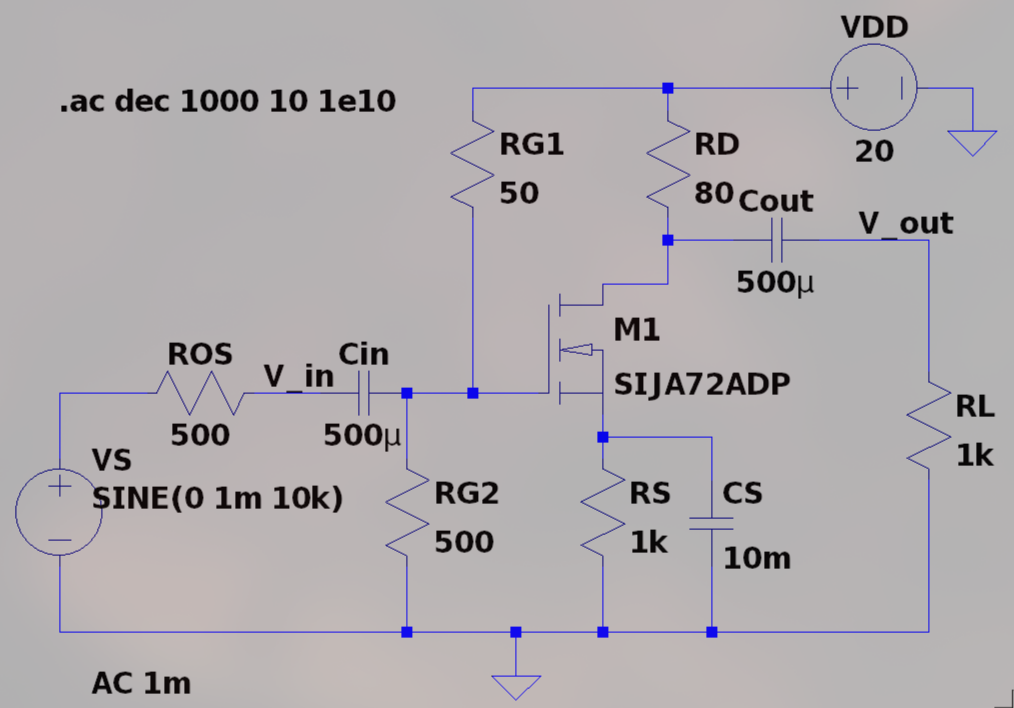
\includegraphics[width=0.7\linewidth]{figs/mosfet_cs_ckt.png}
    \end{figure}
\subsubsection{DC Operating Point}
\begin{figure}[h!]
        \centering
        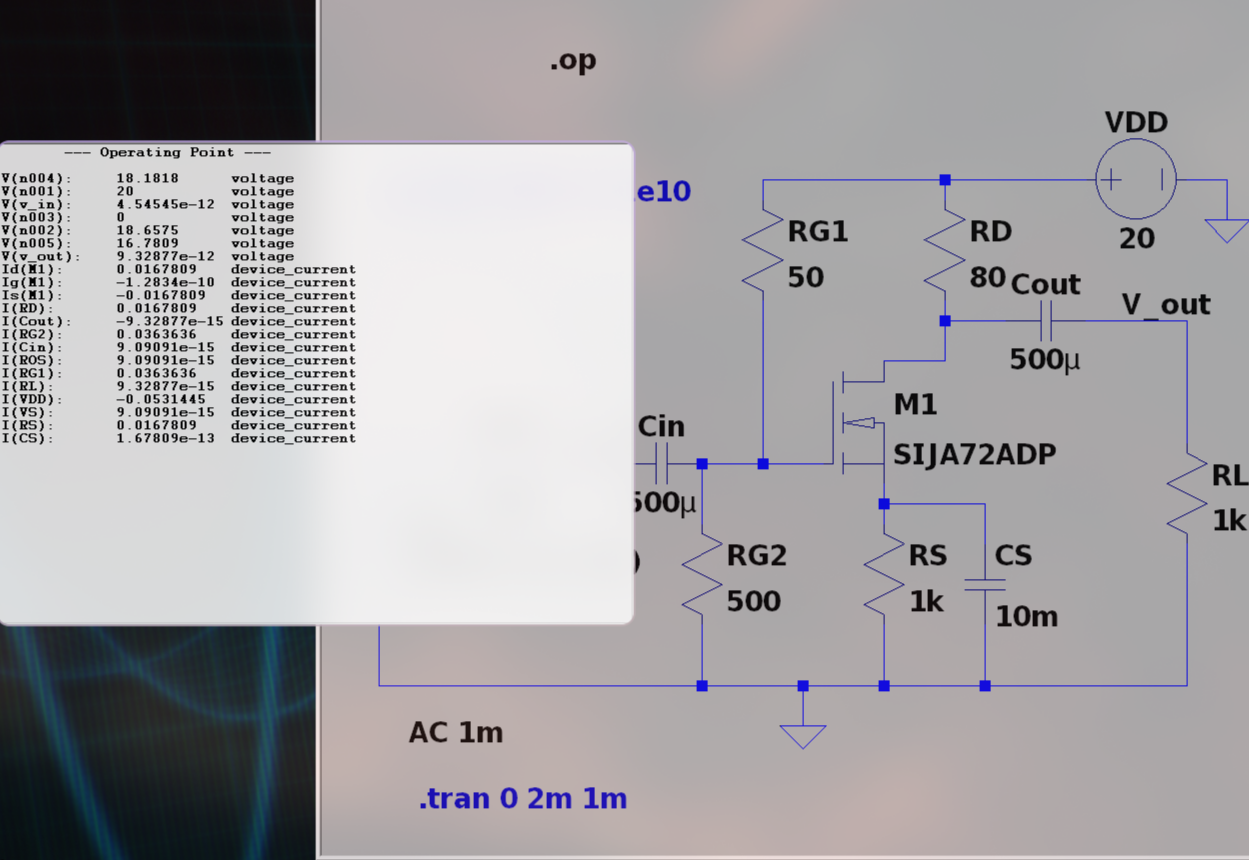
\includegraphics[width=0.7\linewidth]{figs/mosfet_cs_op.png}
    \end{figure}
\pagebreak
\subsubsection{Midband Gain}
\begin{figure}[h!]
        \centering
        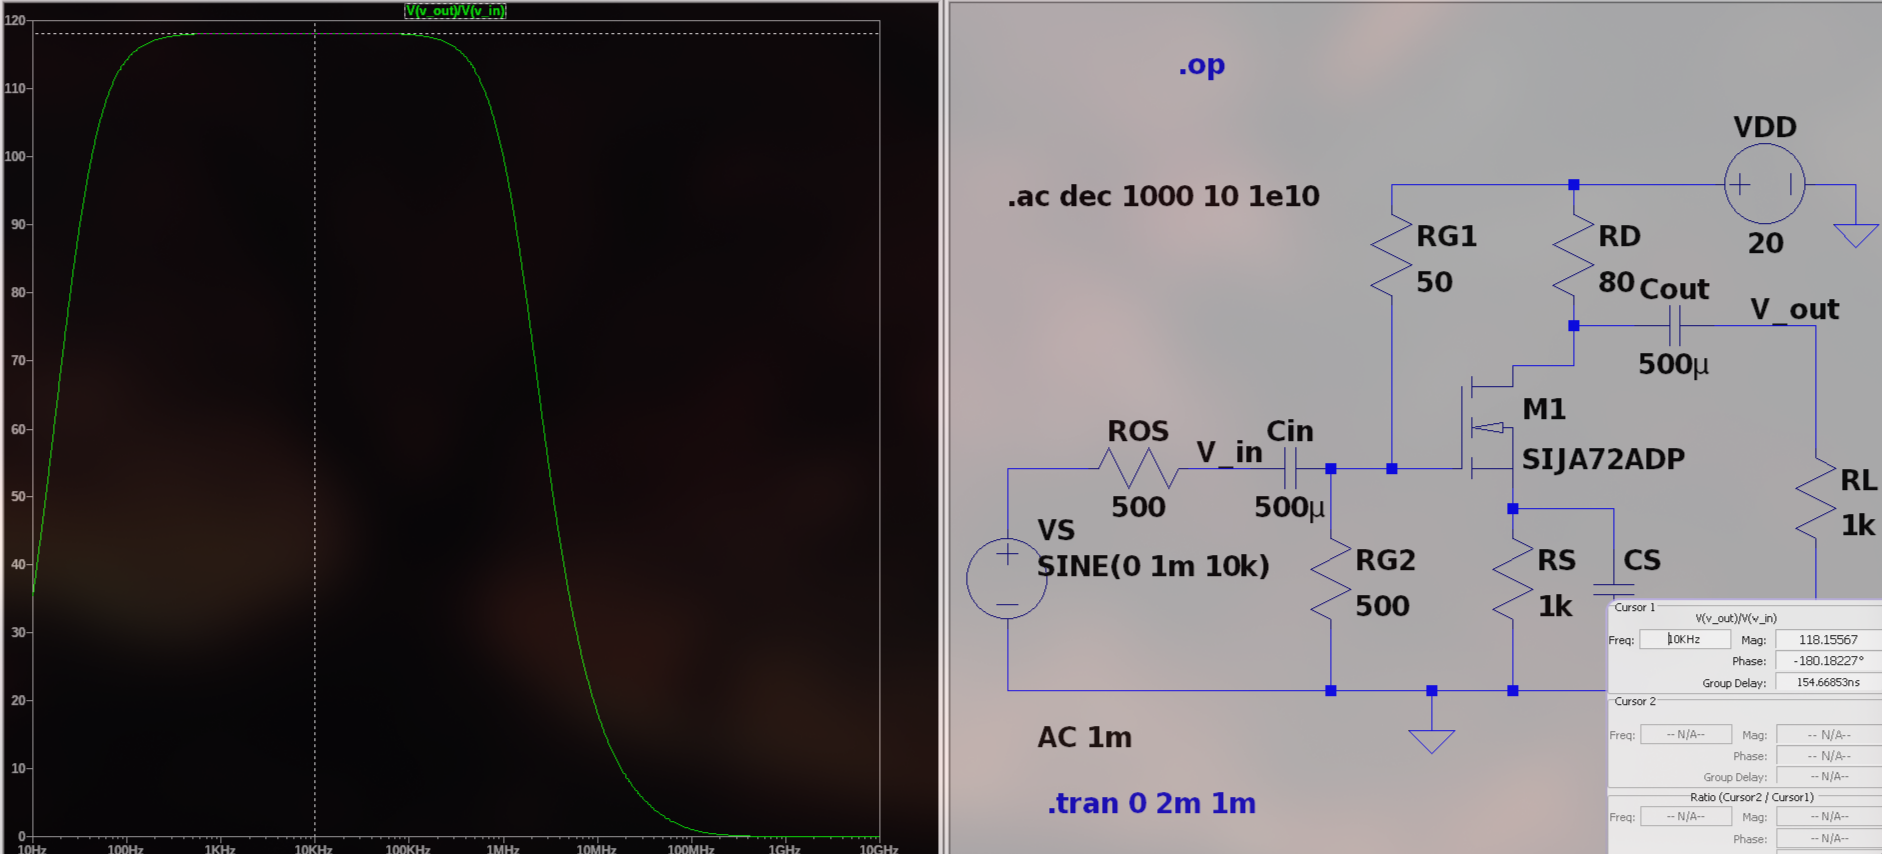
\includegraphics[width=0.7\linewidth]{figs/mosfet_cs_mb.png}
    \end{figure}
\subsubsection{Bandwidth}
\begin{figure}[h!]
        \centering
        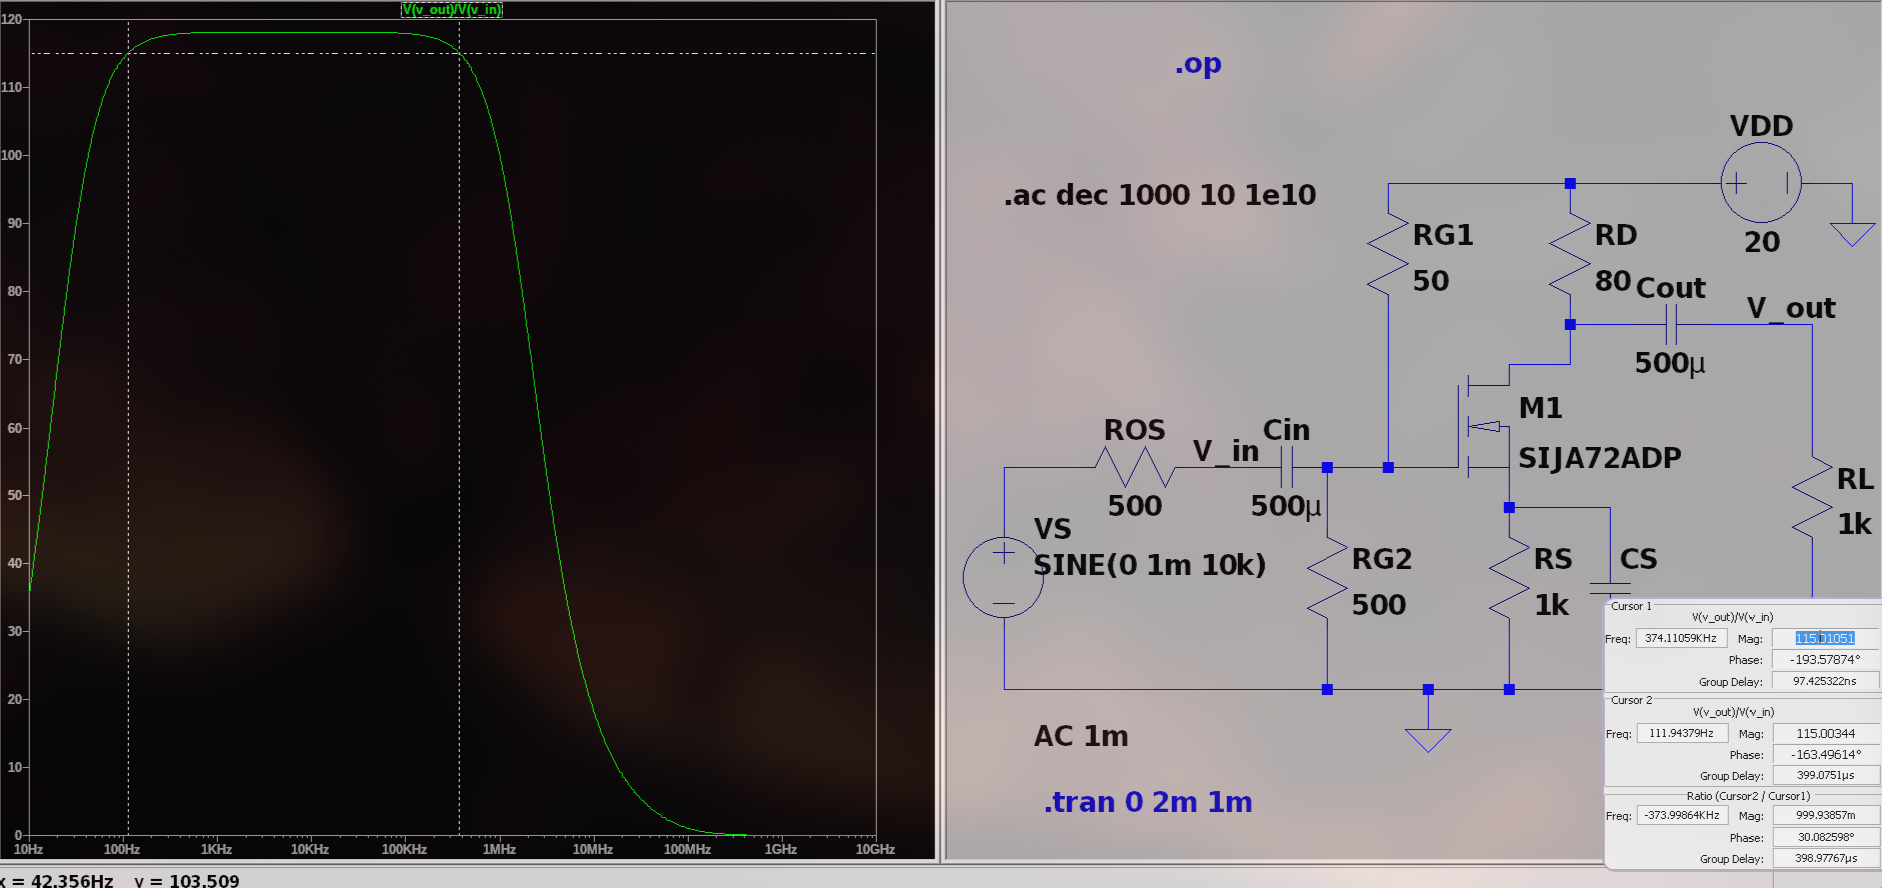
\includegraphics[width=0.7\linewidth]{figs/mosfet_cs_bw.png}
    \end{figure}
\subsubsection{Transient}
\begin{figure}[h!]
        \centering
        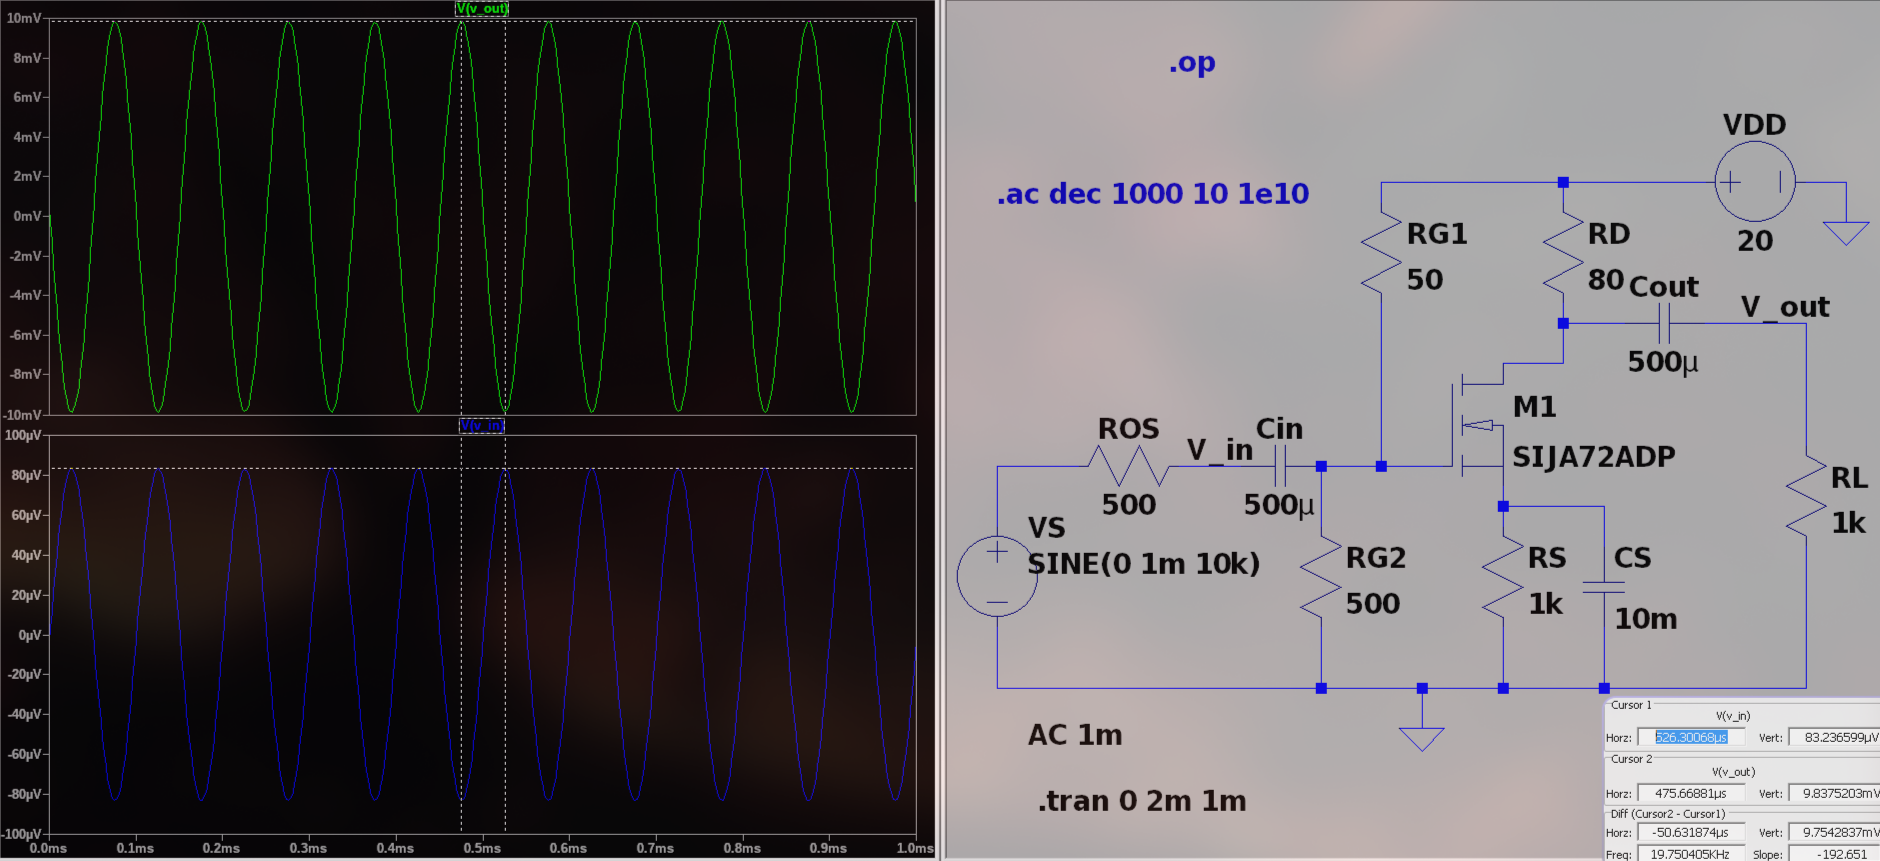
\includegraphics[width=0.7\linewidth]{figs/mosfet_cs_tr.png}
    \end{figure}
    \pagebreak
\subsubsection{Input Resistance}
\begin{figure}[h!]
        \centering
        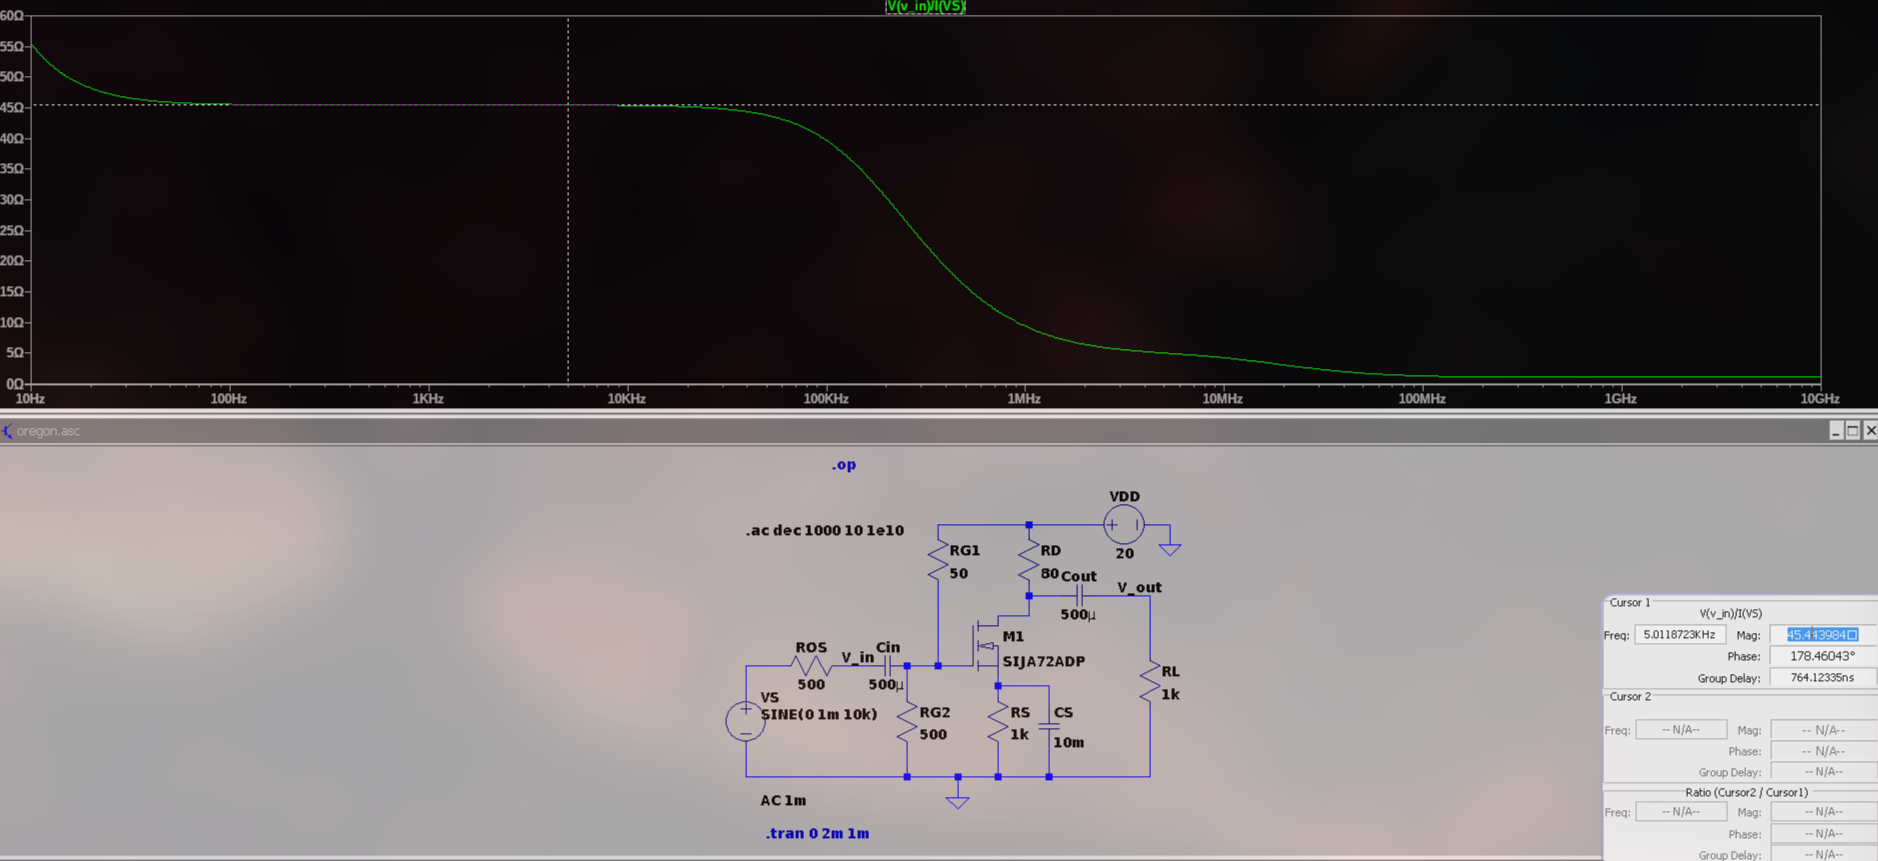
\includegraphics[width=0.7\linewidth]{figs/mosfet_cs_rin.png}
    \end{figure}
\subsubsection{Output Resistance}
\begin{figure}[h!]
        \centering
        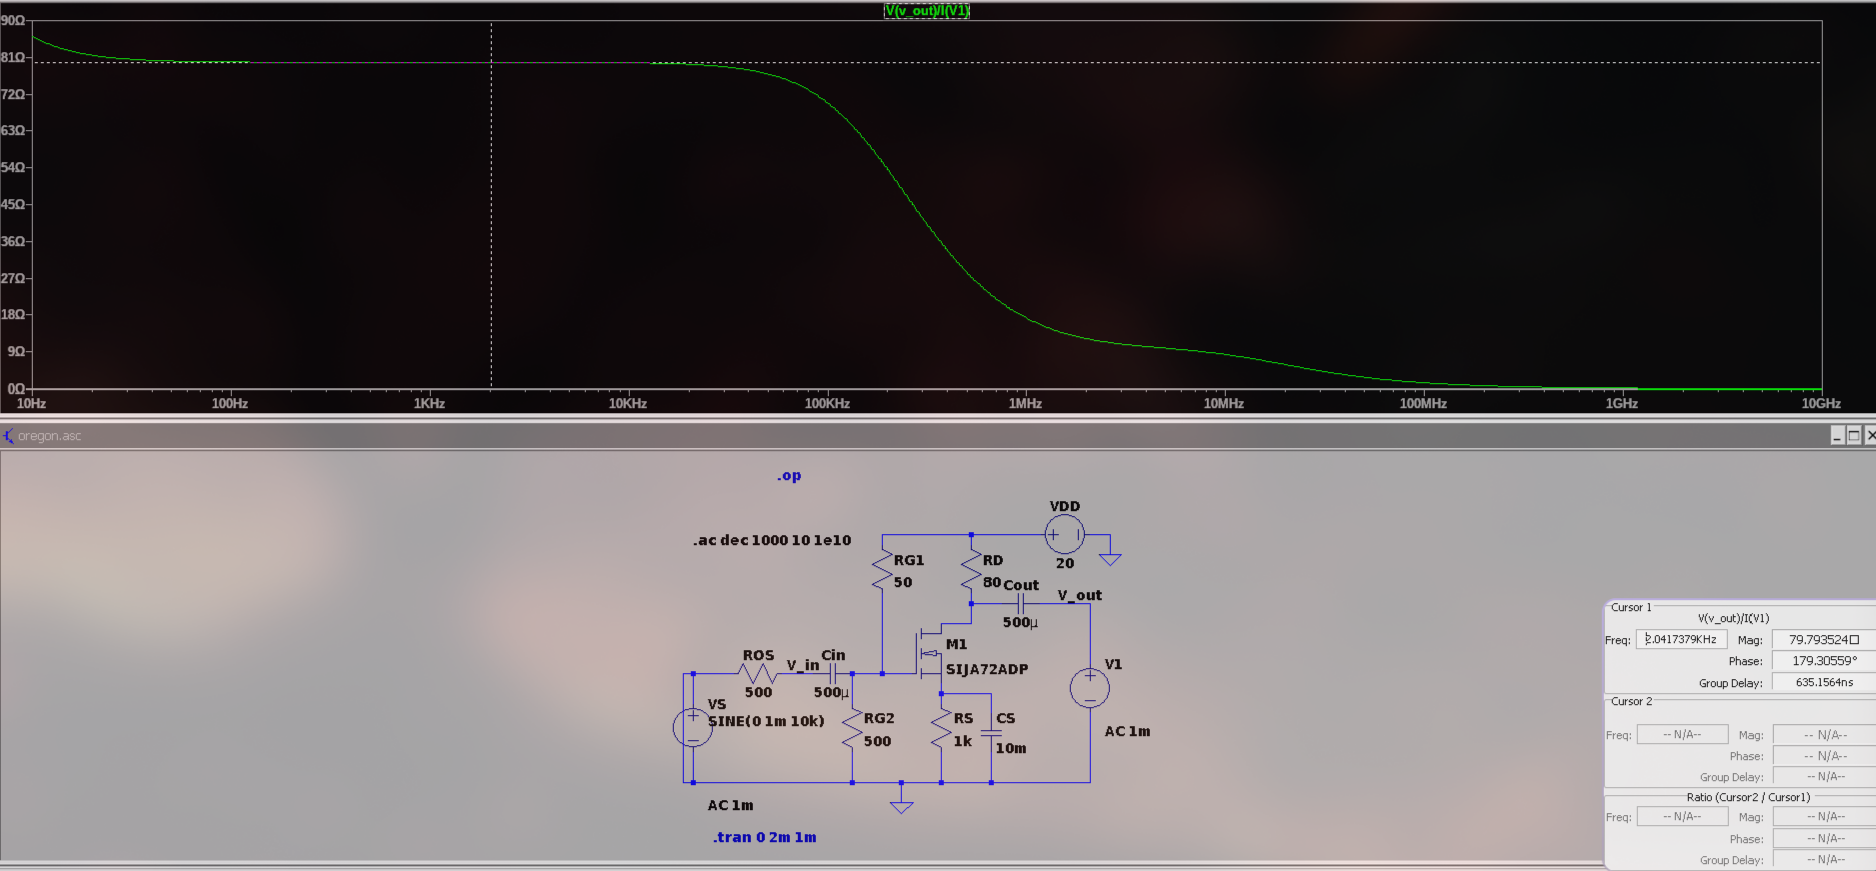
\includegraphics[width=0.7\linewidth]{figs/mosfet_cs_rout.png}
    \end{figure}
\subsubsection{Theory}
\begin{enumerate}
    \item Transconductance $g_m = \frac{2I_d}{V_{GS}-V_{TO}}$ 
    \item $V_{TO} = 1.38V$ (Specific to MOSFET model)
    \item Input Resistance $R_i = R_{G1} \parallel R_{G2}$  
    \item Output Resistance $R_o = R_D $ 
    \item Voltage gain $A = \frac{V_{in}}{V_{out}} = g_m R_o$ 
\end{enumerate} 
\subsection{Data}
\begin{tabular}{|c|c|c|c|c|c|c|}
\hline
\makecell{\textbf{Midband gain} \\ \textbf{(graph)}} & \makecell{\textbf{Midband gain} \\ \textbf{(theory)}} & \makecell{$\mathbf{R_i}$ \\ \textbf{(graph)}} & \makecell{{$\mathbf{R_i}$} \\ \textbf{(theory)}} & \makecell{{$\mathbf{R_o}$} \\ \textbf{(graph)}} & \makecell{{$\mathbf{R_o}$} \\ \textbf{(theory)}} & \textbf{Bandwidth} \\
\hline
$118.15567$ & $123.155$ & $45.443984\Omega$ & $45.4545 \Omega$& $79.793524 \Omega$ & $80 \Omega$ & $373.9986$ KHz \\
\hline
\end{tabular}

\pagebreak
\subsection{Common Drain}
\subsubsection{Circuit}
\begin{figure}[h!]
        \centering
        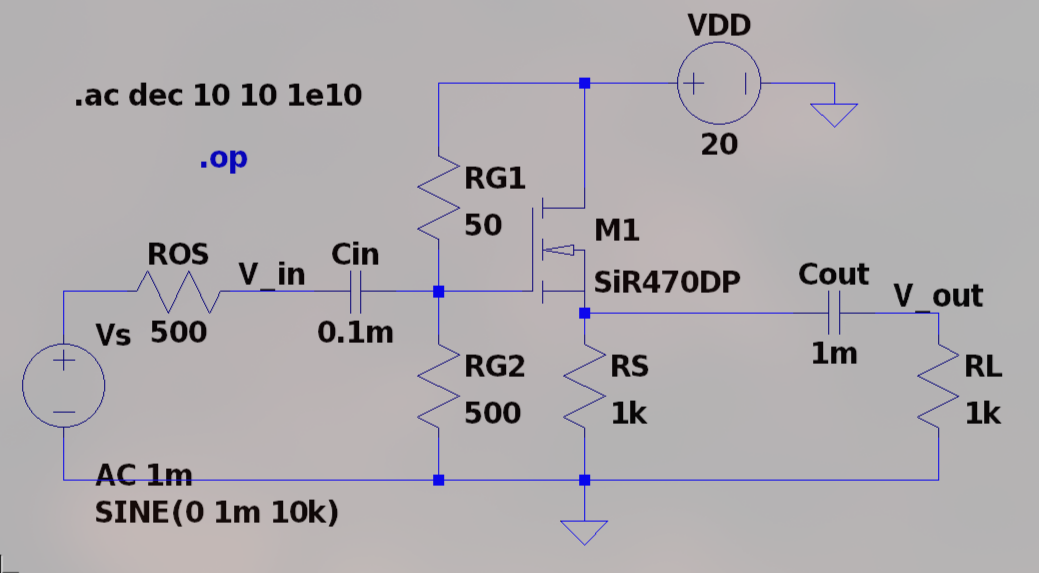
\includegraphics[width=0.7\linewidth]{figs/mosfet_cd_ckt.png}
    \end{figure}
\subsubsection{DC Operating Point}
\begin{figure}[h!]
        \centering
        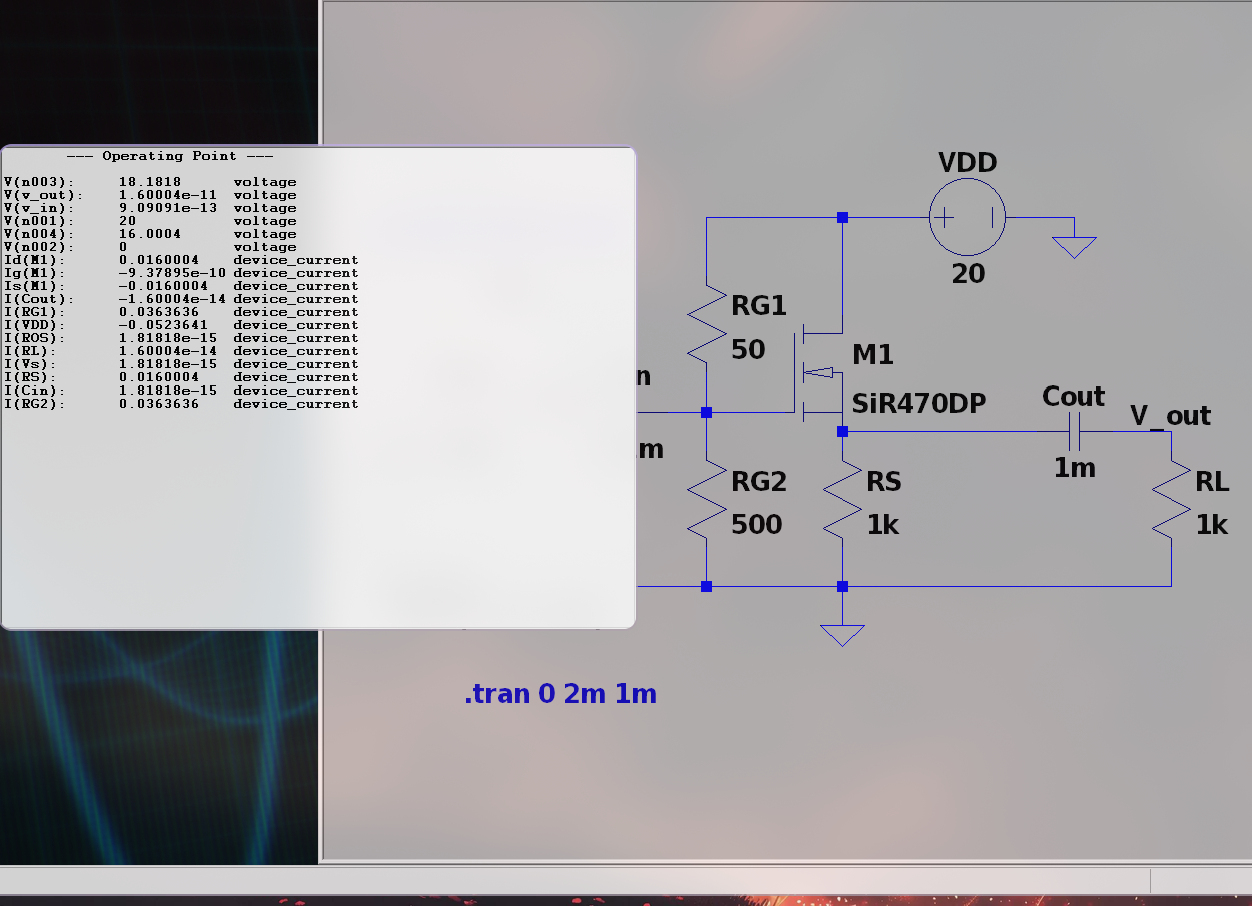
\includegraphics[width=0.7\linewidth]{figs/mosfet_cd_op.png}
    \end{figure}
\pagebreak
\subsubsection{Midband Gain}
\begin{figure}[h!]
        \centering
        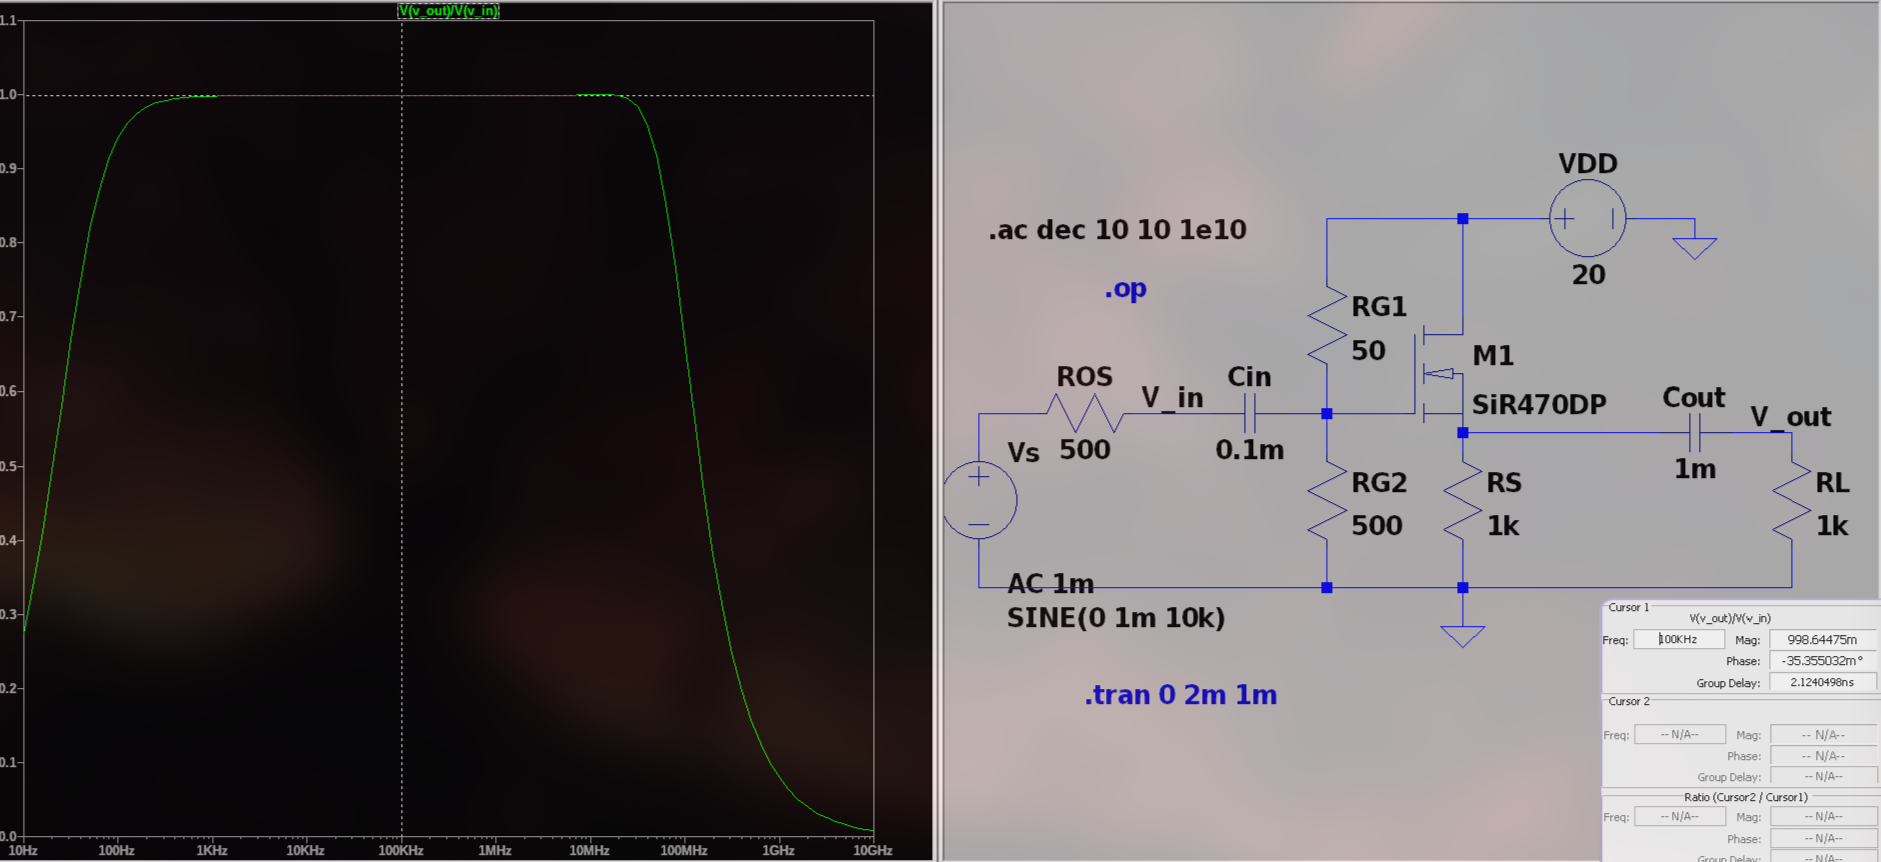
\includegraphics[width=0.7\linewidth]{figs/mosfet_cd_mb.png}
    \end{figure}
\subsubsection{Bandwidth}
\begin{figure}[h!]
        \centering
        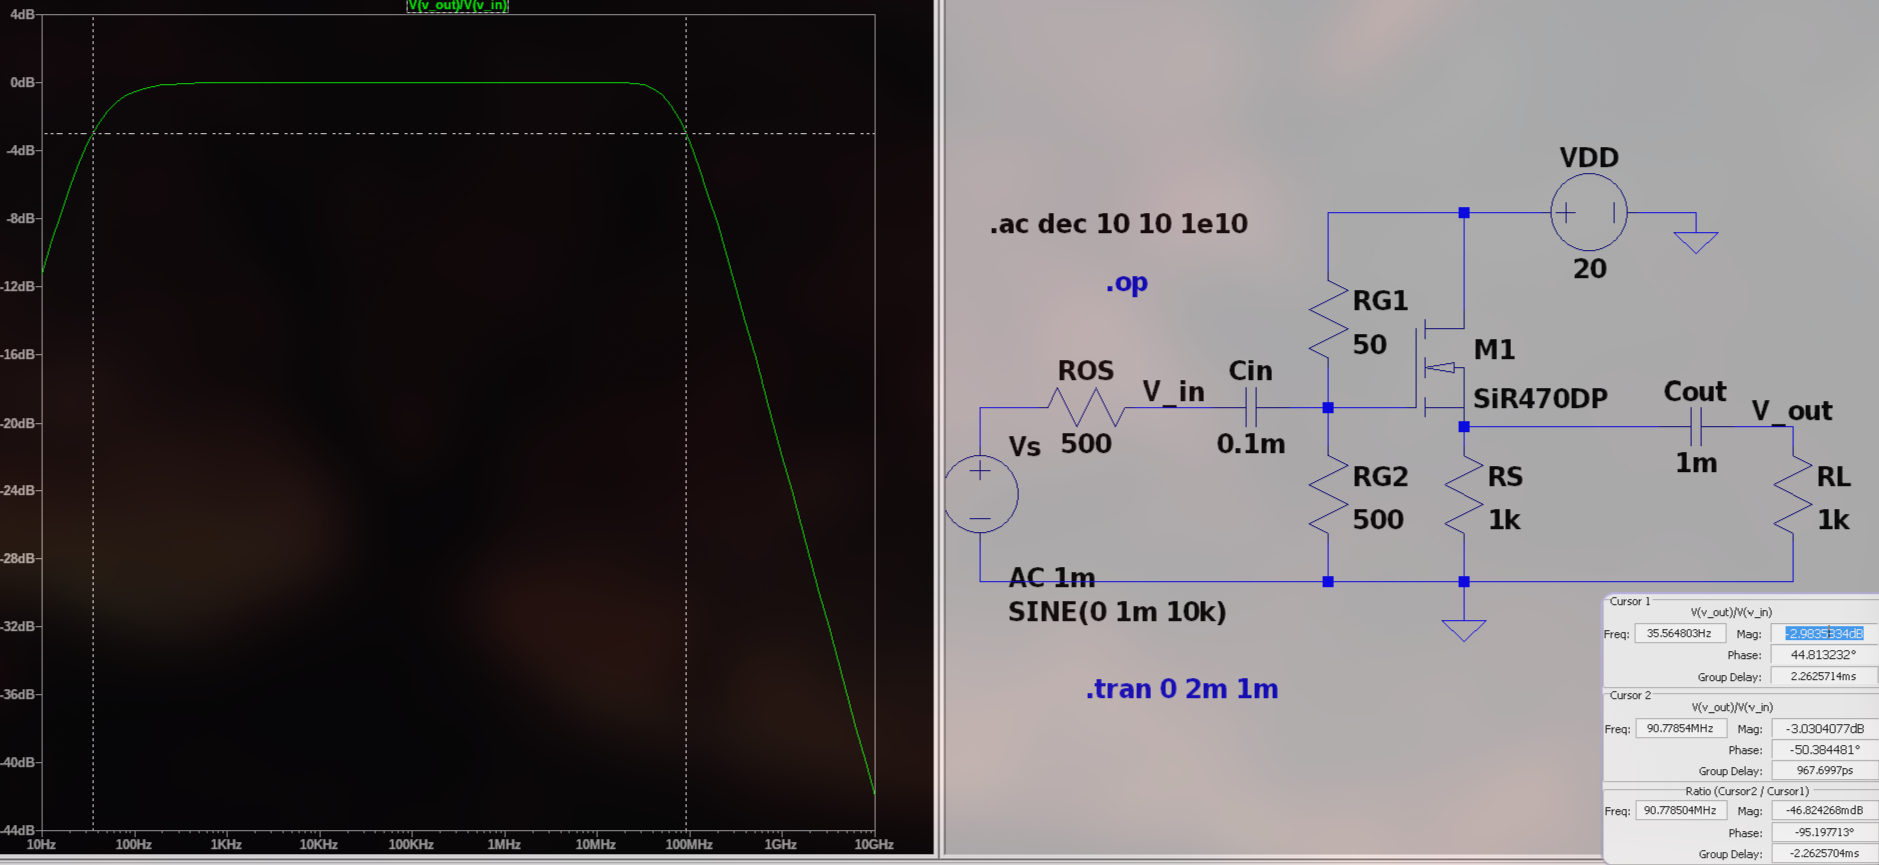
\includegraphics[width=0.7\linewidth]{figs/mosfet_cd_bw.png}
    \end{figure}
\subsubsection{Transient}
\begin{figure}[h!]
        \centering
        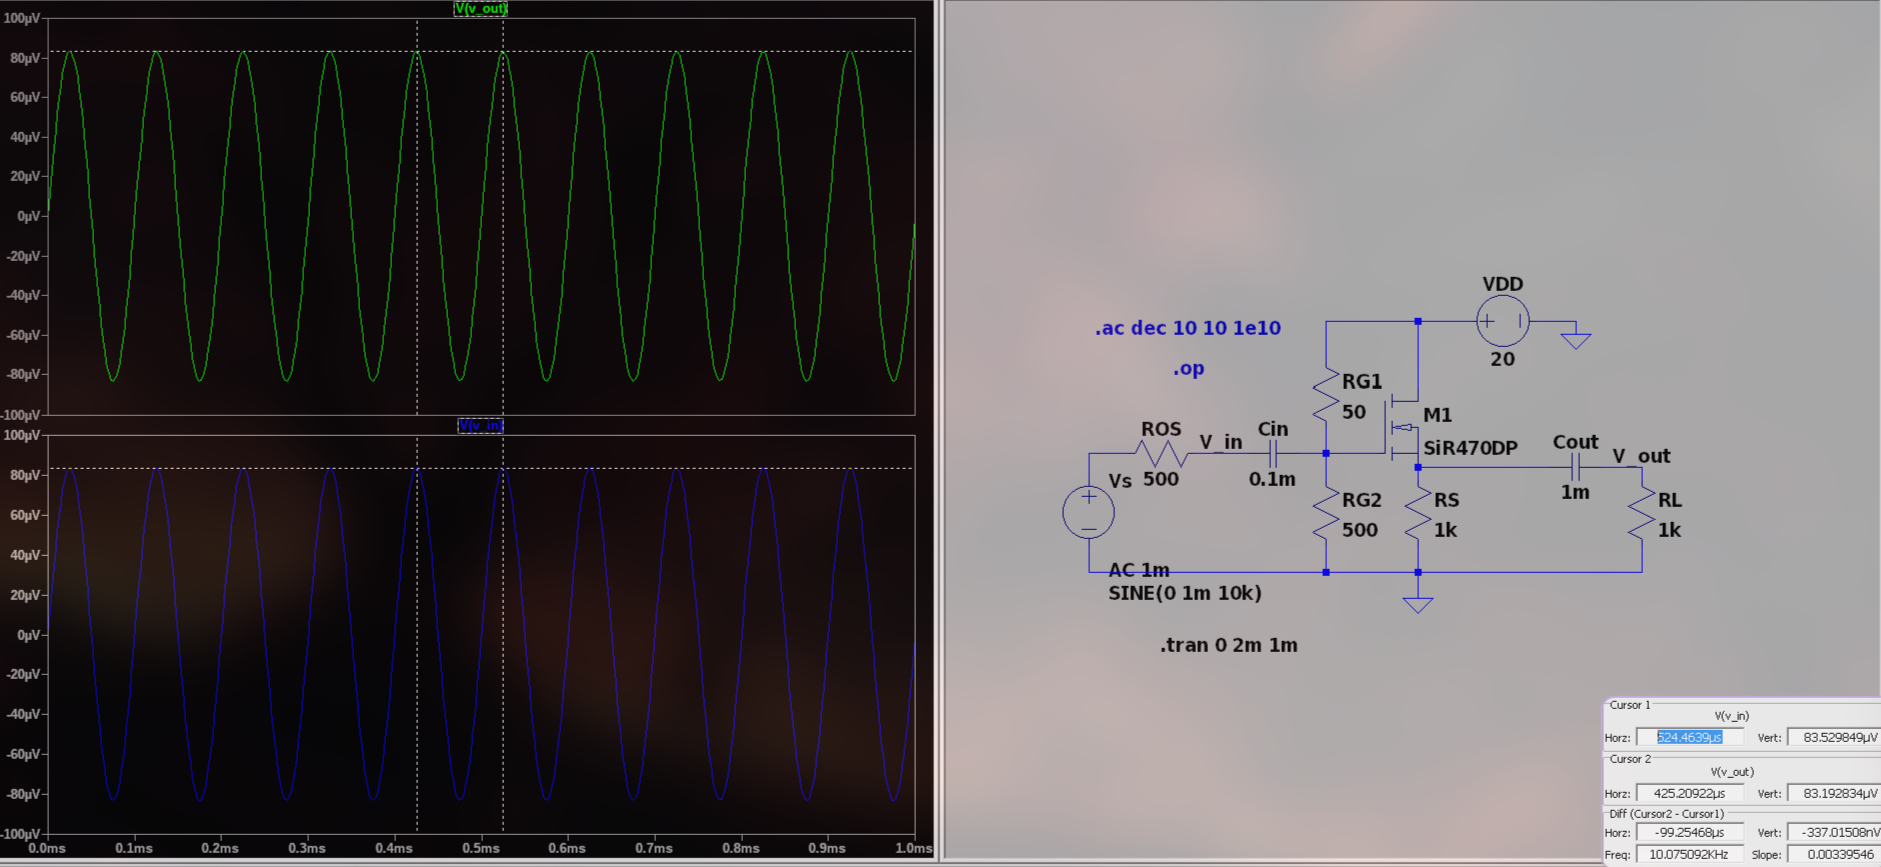
\includegraphics[width=0.7\linewidth]{figs/mosfet_cd_tr.png}
    \end{figure}
    \pagebreak
\subsubsection{Input Resistance}
\begin{figure}[h!]
        \centering
        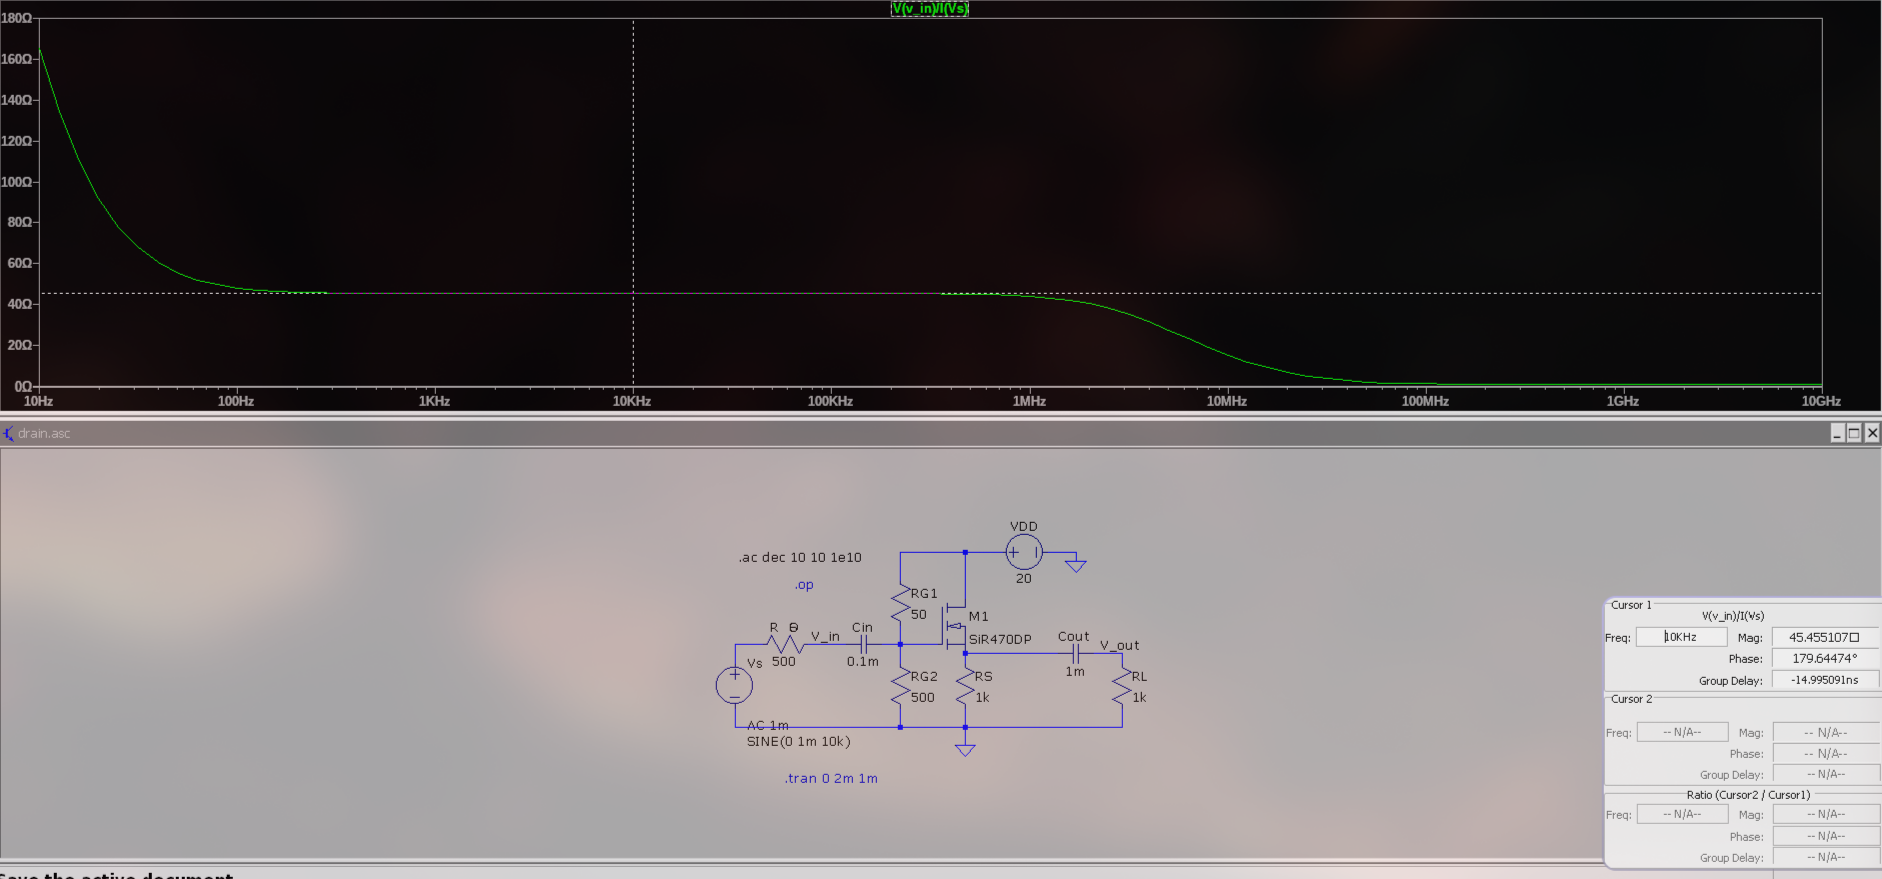
\includegraphics[width=0.7\linewidth]{figs/mosfet_cd_rin.png}
    \end{figure}
\subsubsection{Output Resistance}
\begin{figure}[h!]
        \centering
        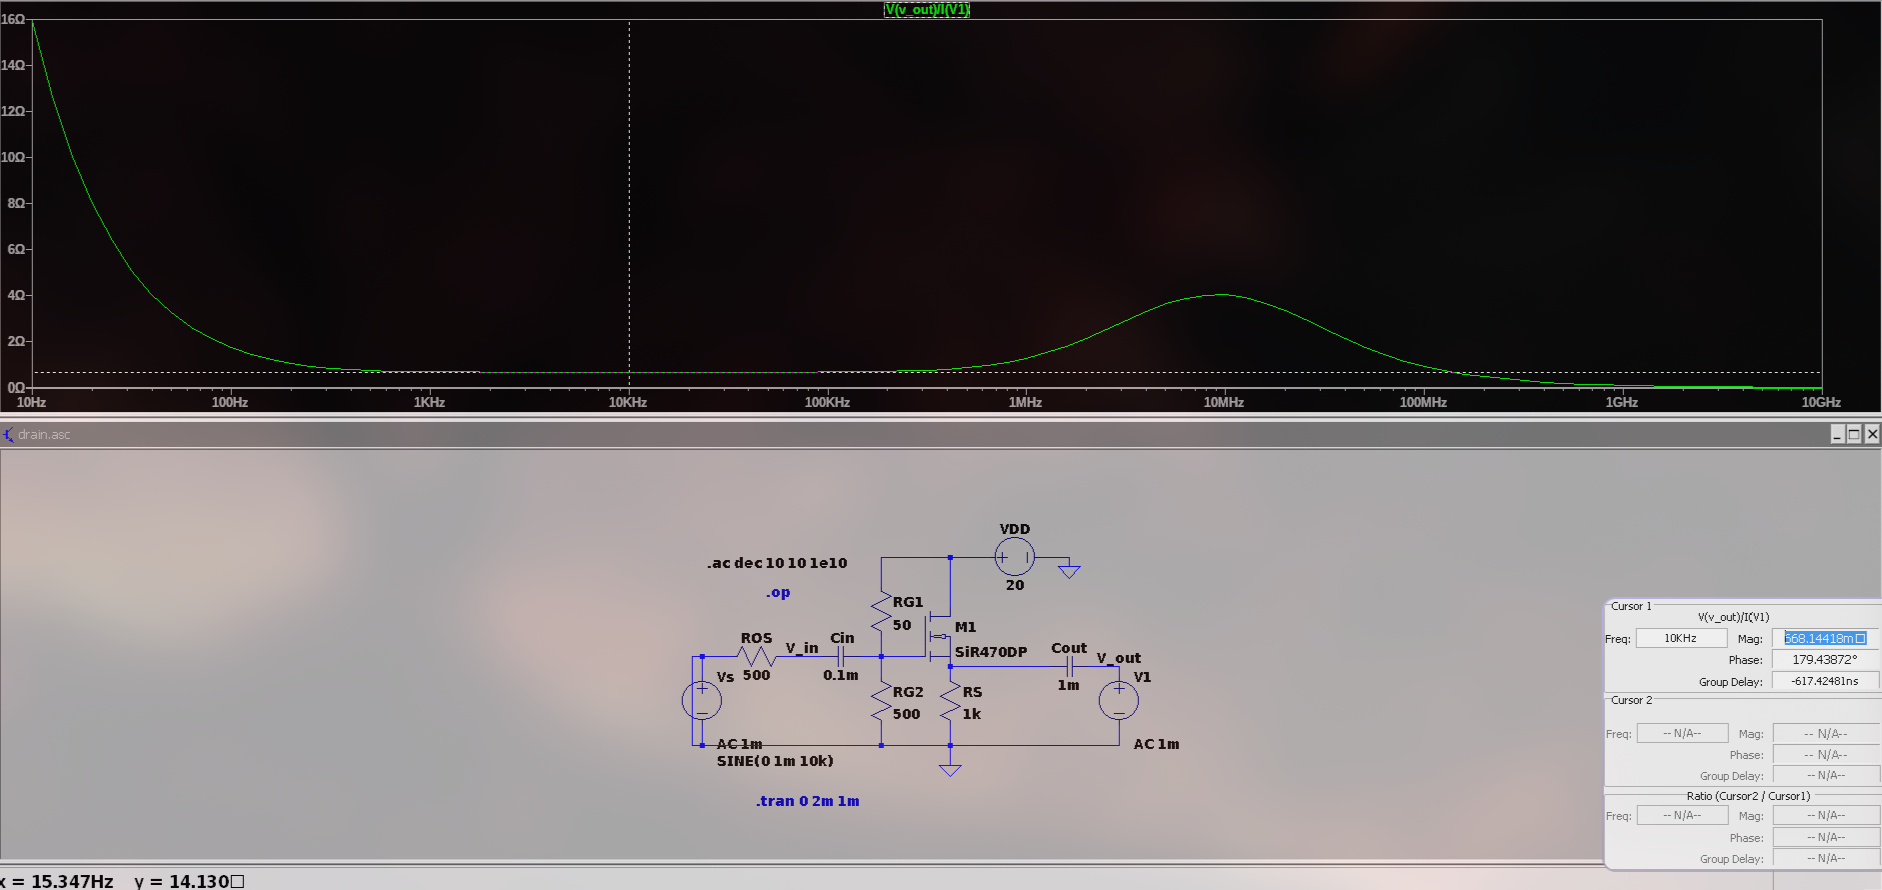
\includegraphics[width=0.7\linewidth]{figs/mosfet_cd_rout.png}
    \end{figure}
\subsubsection{Theory}
\begin{enumerate}
    \item Transconductance $g_m = \frac{2I_d}{V_{GS}-V_{TO}}$ 
    \item $V_{TO} = 2.16V$ (Specific to MOSFET model)
    \item Input Resistance $R_i = R_{G1} \parallel R_{G2}$  
    \item Output Resistance $R_o = R_S \parallel \frac{1}{g_m} $ 
    \item Voltage gain $A = \frac{V_{in}}{V_{out}} = \frac{gm \brak{R_s \parallel R_L}}{1+gm \brak{R_s \parallel R_L}}$ 
\end{enumerate} 
\subsubsection{Data}
\begin{tabular}{|c|c|c|c|c|c|c|}
\hline
\makecell{\textbf{Midband gain} \\ \textbf{(graph)}} & \makecell{\textbf{Midband gain} \\ \textbf{(theory)}} & \makecell{$\mathbf{R_i}$ \\ \textbf{(graph)}} & \makecell{{$\mathbf{R_i}$} \\ \textbf{(theory)}} & \makecell{{$\mathbf{R_o}$} \\ \textbf{(graph)}} & \makecell{{$\mathbf{R_o}$} \\ \textbf{(theory)}} & \textbf{Bandwidth} \\
\hline
$0.99864$ & $0.998638$ & $45.45510\Omega$ & $45.4545 \Omega$& $0.668144 \Omega$ & $0.68134\Omega$ & $90.7785 MHz$ \\
\hline
\end{tabular}
\pagebreak
\subsection{Common Gate}
\subsubsection{Circuit}
\begin{figure}[h!]
        \centering
        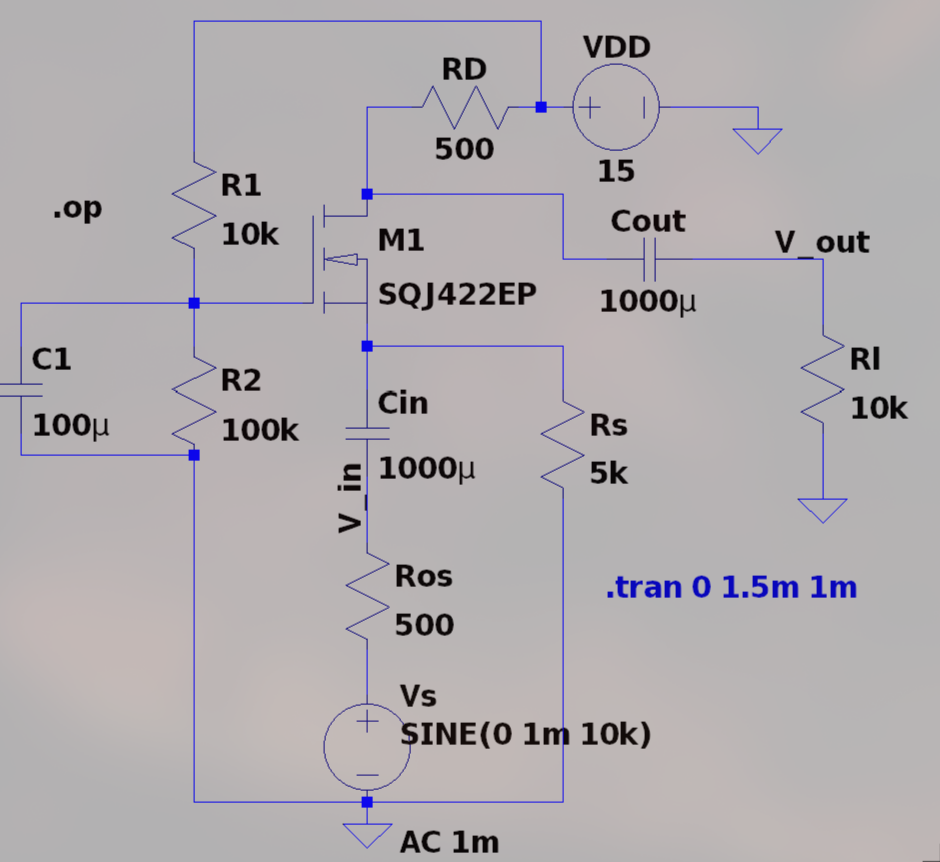
\includegraphics[width=0.7\linewidth]{figs/mosfet_cg_ckt.png}
    \end{figure}
\subsubsection{DC Operating Point}
\begin{figure}[h!]
        \centering
        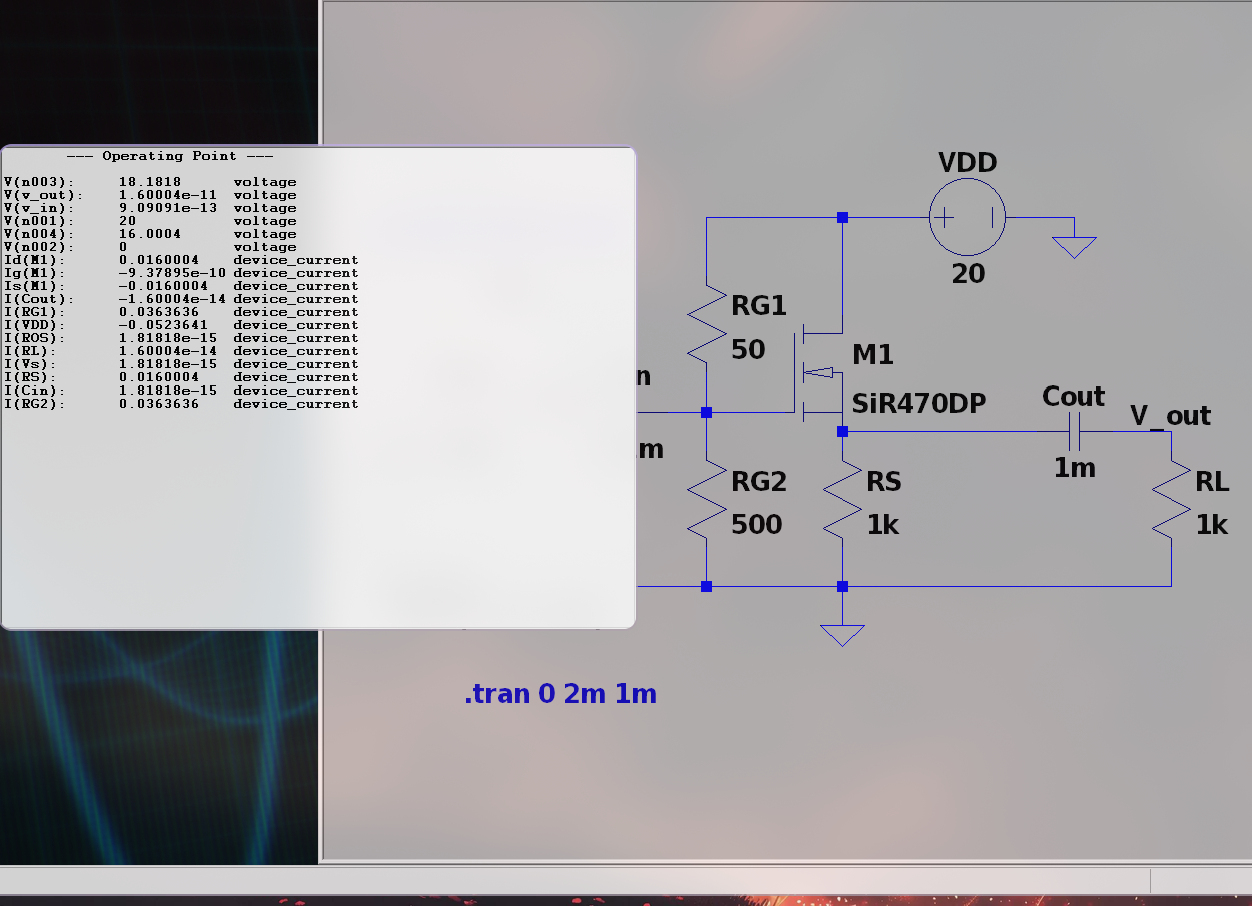
\includegraphics[width=0.7\linewidth]{figs/mosfet_cd_op.png}
    \end{figure}
\pagebreak
\subsubsection{Midband Gain}
\begin{figure}[h!]
        \centering
        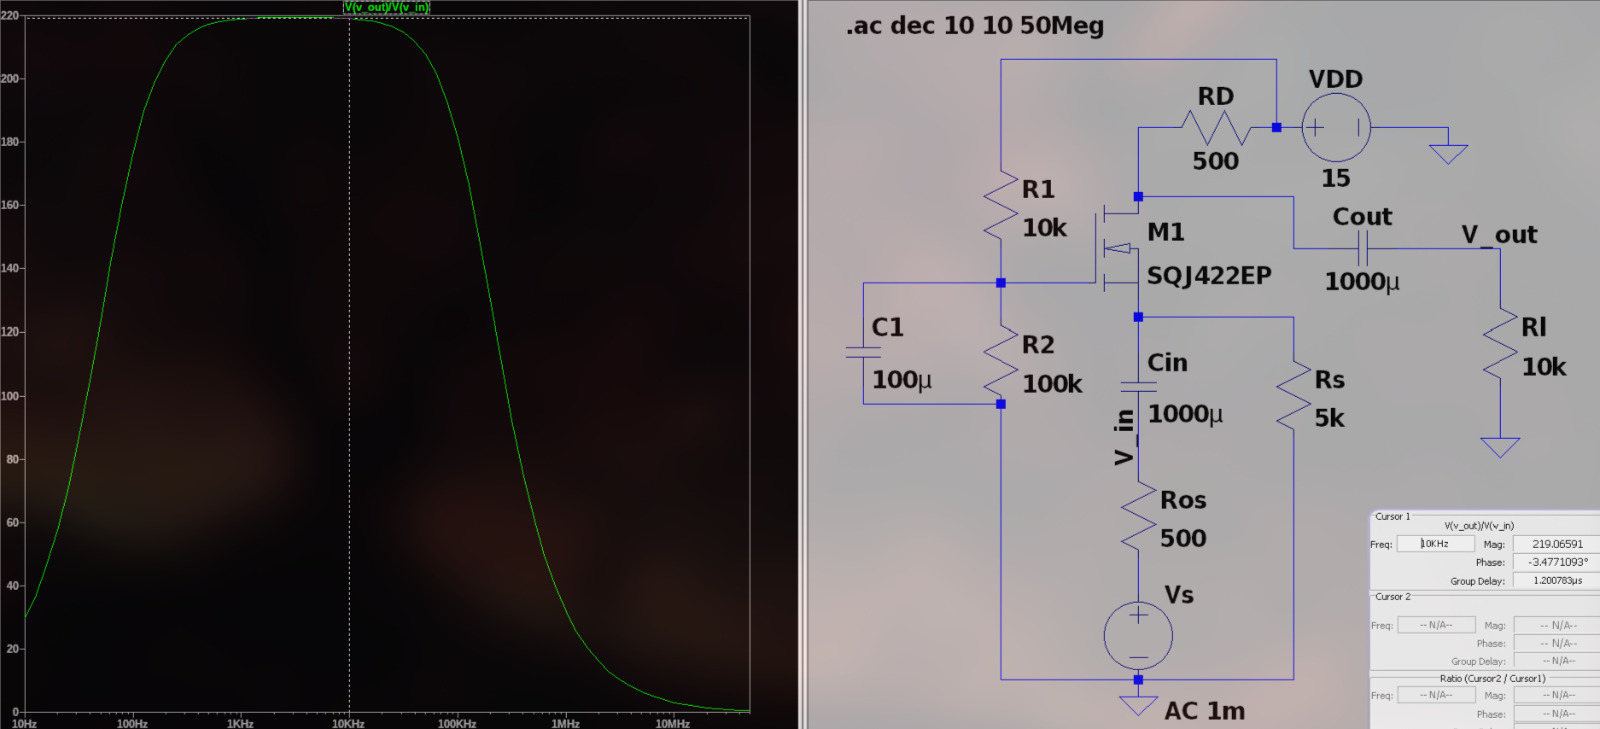
\includegraphics[width=0.7\linewidth]{figs/mosfet_cg_mb.png}
    \end{figure}
\subsubsection{Bandwidth}
\begin{figure}[h!]
        \centering
        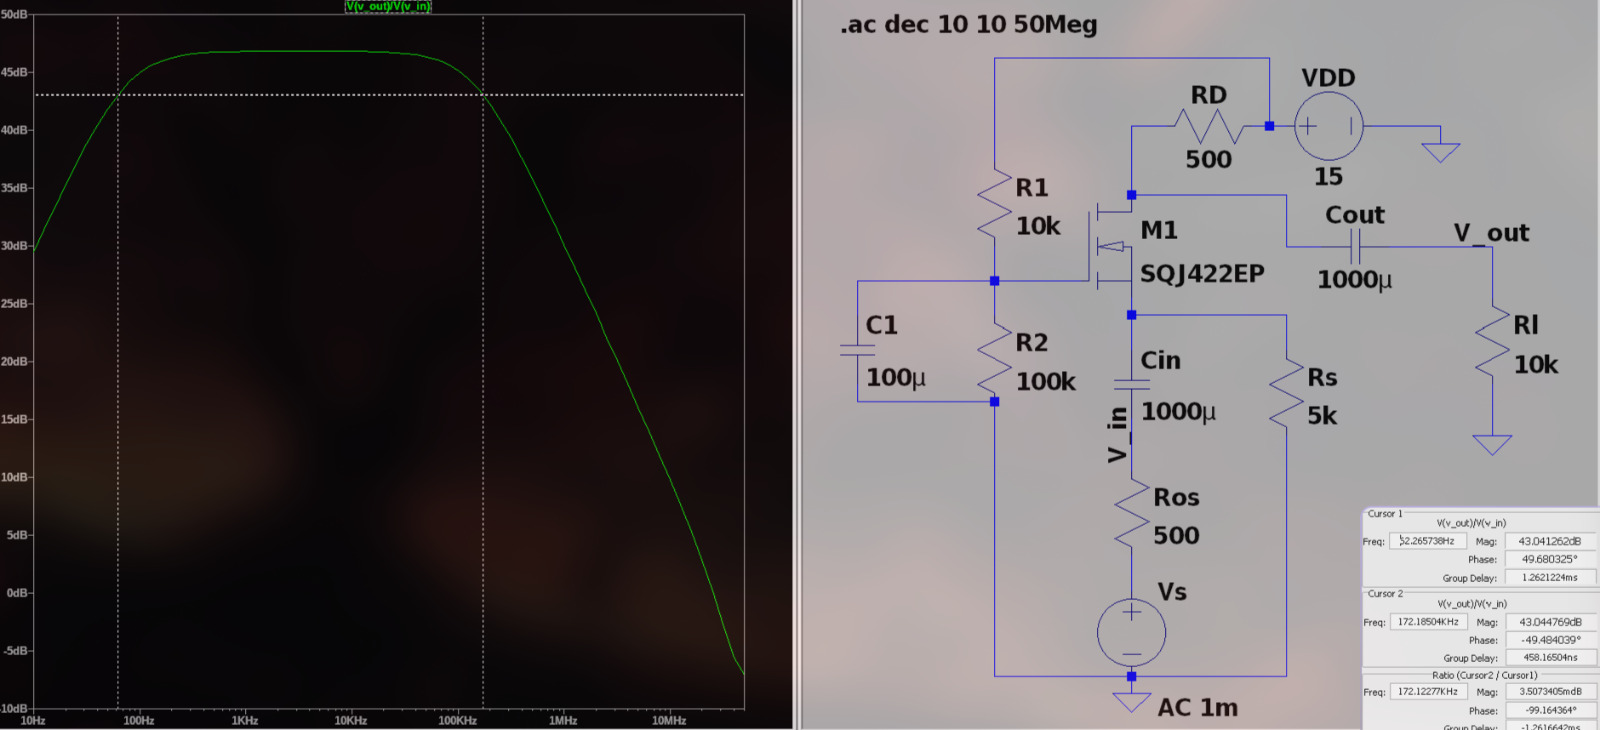
\includegraphics[width=0.7\linewidth]{figs/mosfet_cg_bw.png}
    \end{figure}
\subsubsection{Transient}
\begin{figure}[h!]
        \centering
        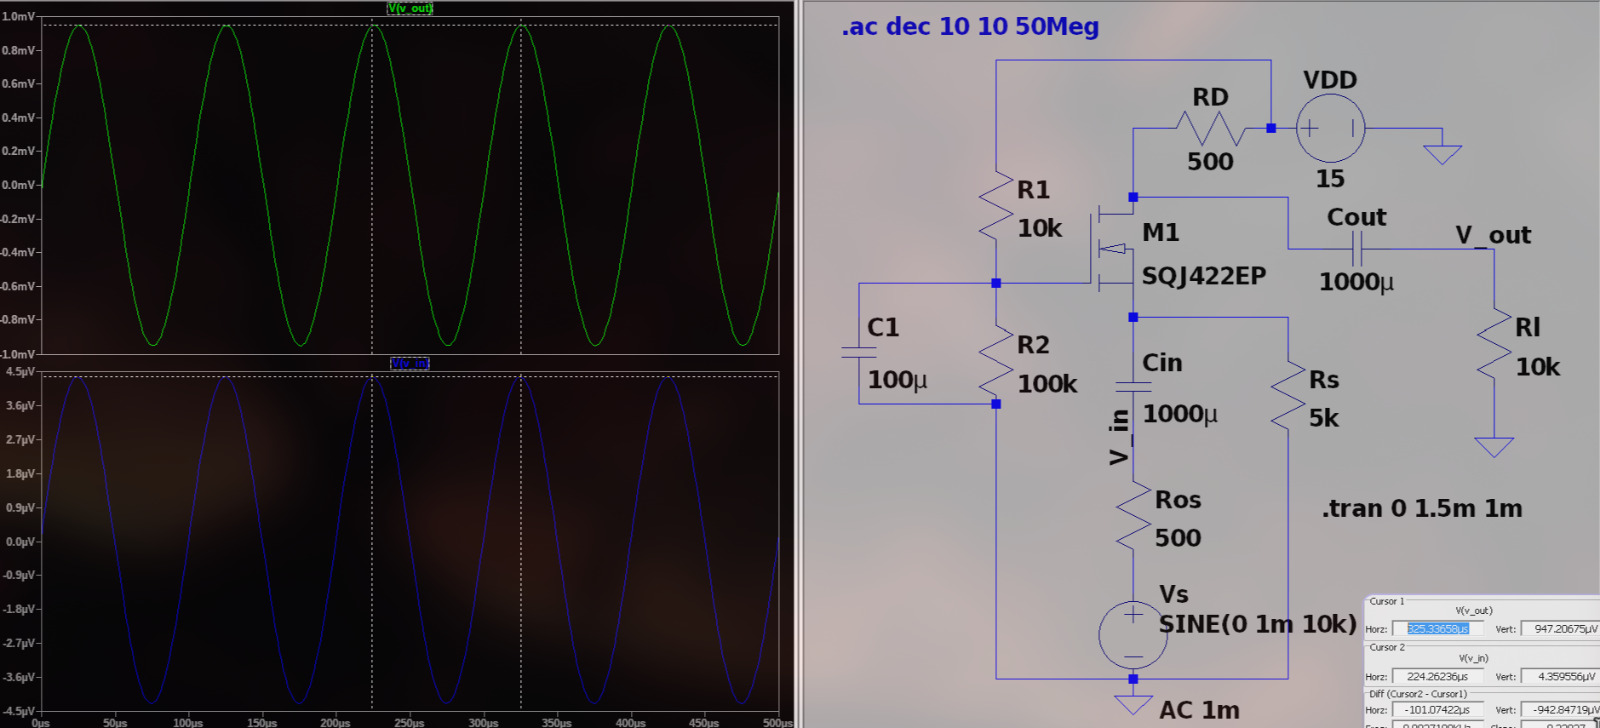
\includegraphics[width=0.7\linewidth]{figs/mosfet_cg_tr.png}
    \end{figure}
    \pagebreak
\subsubsection{Input Resistance}
\begin{figure}[h!]
        \centering
        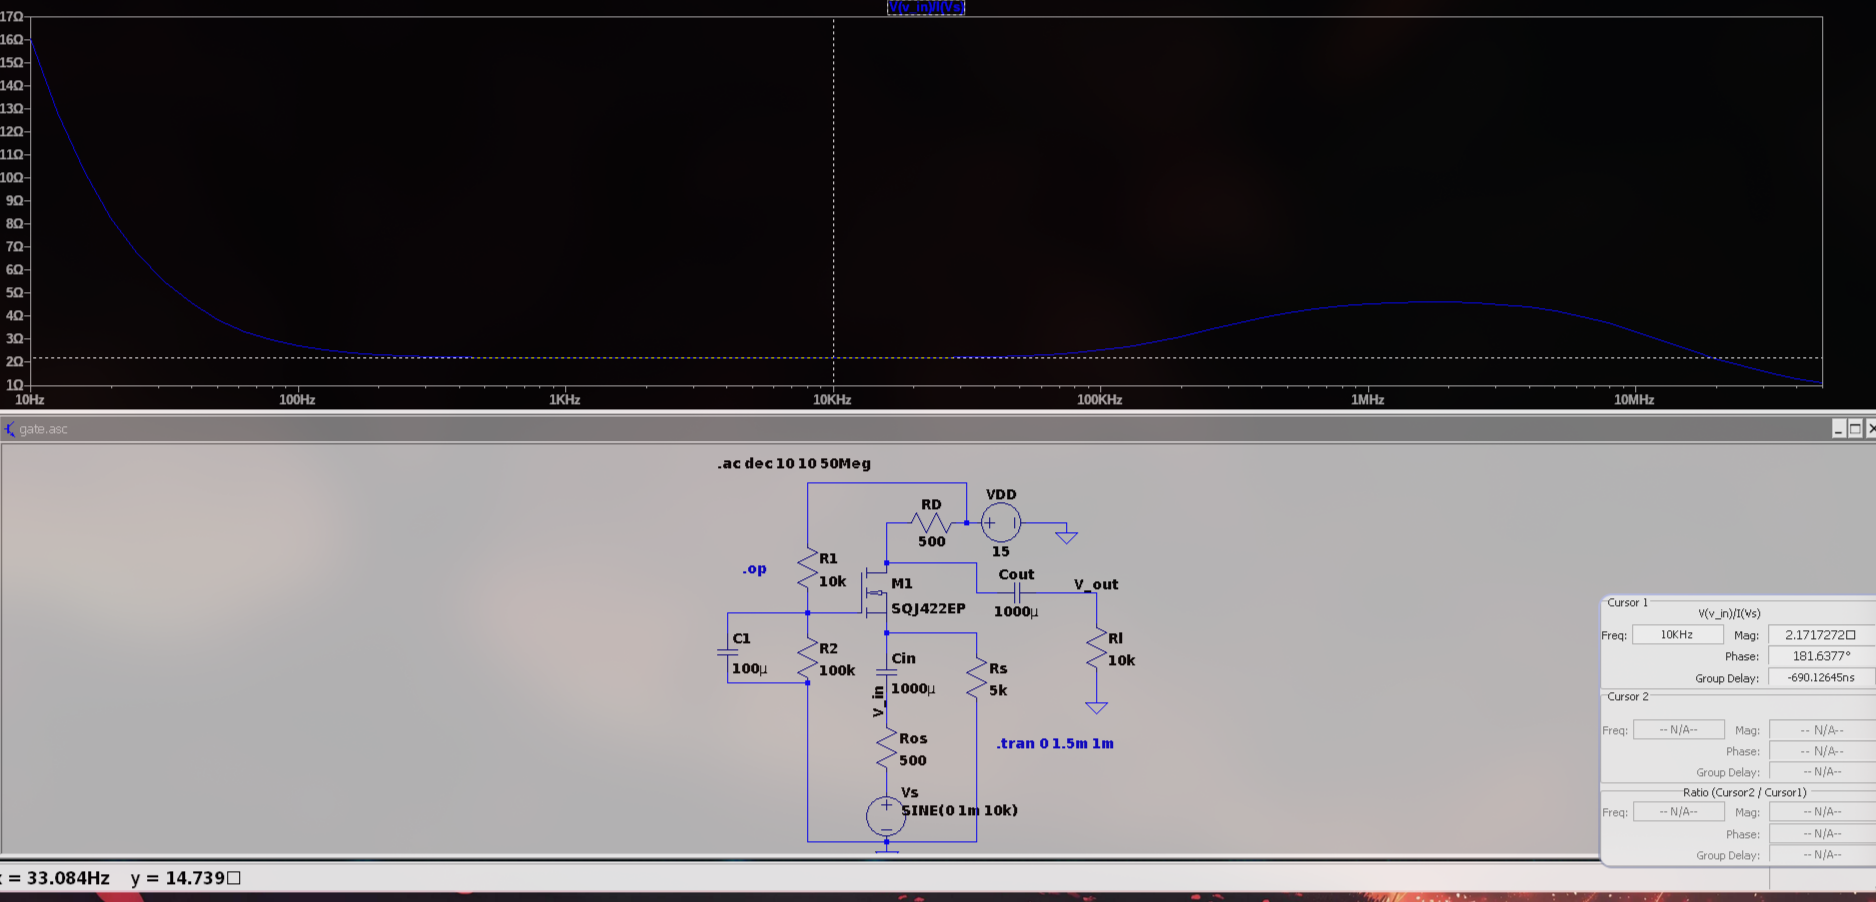
\includegraphics[width=0.7\linewidth]{figs/mosfet_cg_rin.png}
    \end{figure}
\subsubsection{Output Resistance}
\begin{figure}[h!]
        \centering
        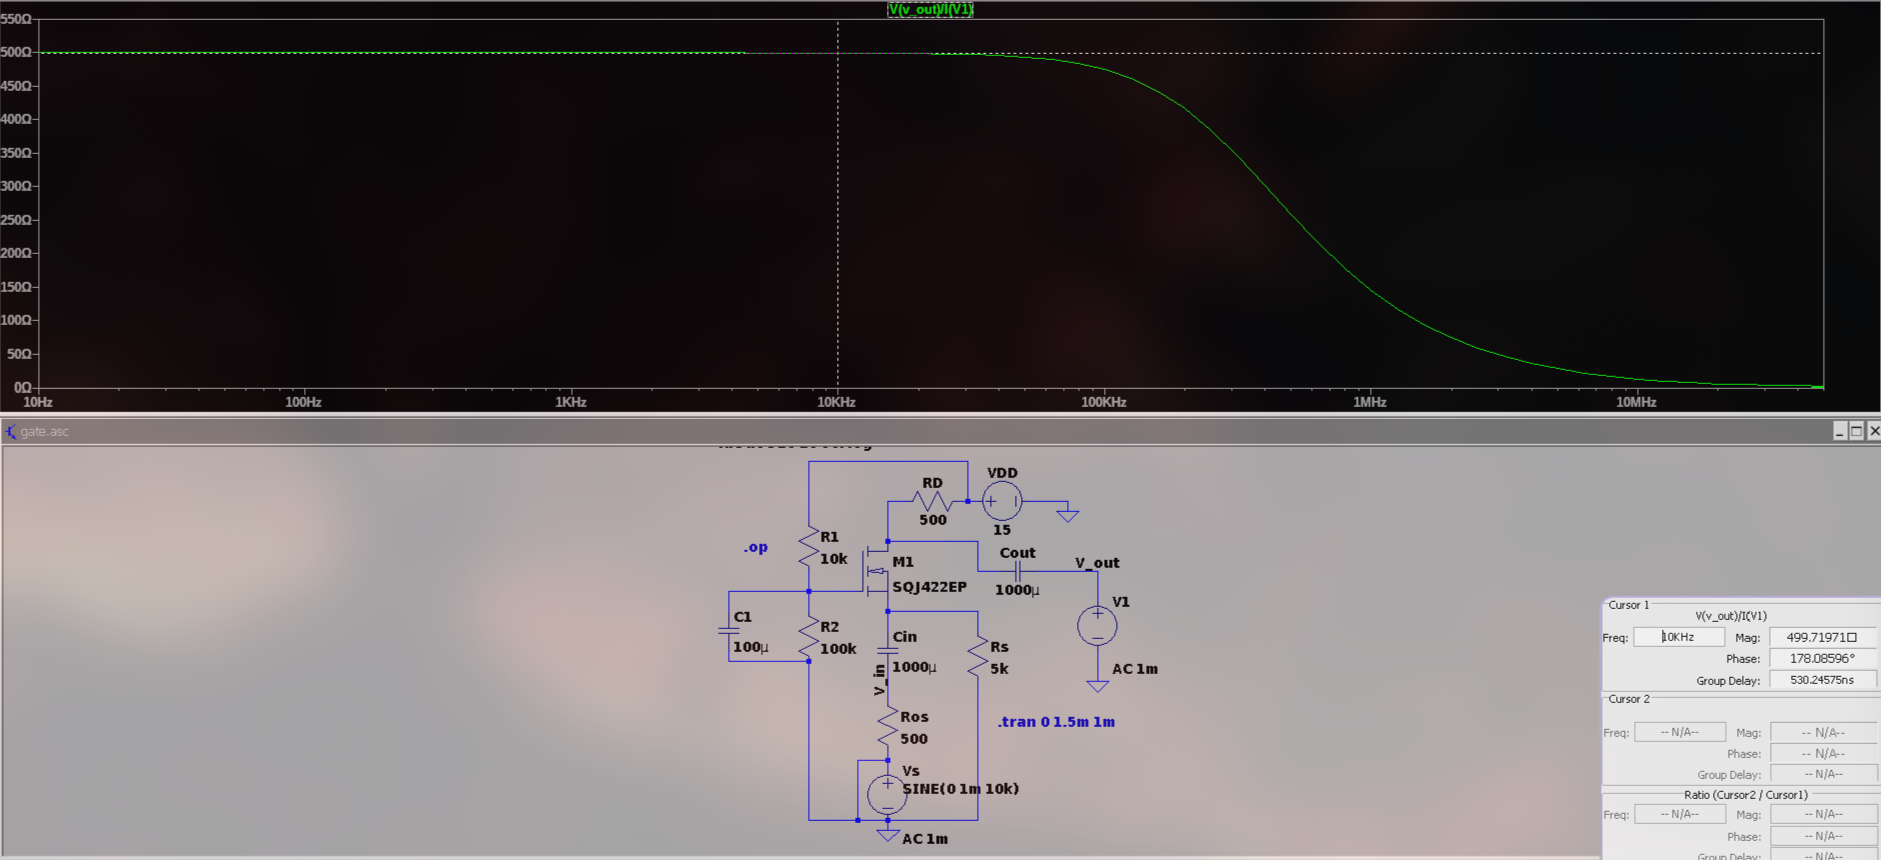
\includegraphics[width=0.7\linewidth]{figs/mosfet_cg_rout.png}
    \end{figure}

\subsubsection{Theory}
\begin{enumerate}
    \item Transconductance $g_m = \frac{2I_d}{V_{GS}-V_{TO}}$
    \item $V_{TO} = 2.16V$ (Specific to MOSFET model)
    \item Input Resistance $R_i = R_{S} \parallel \frac{1}{g_m}$  
    \item Output Resistance $R_o = R_D $ 
    \item Voltage gain $A = \frac{V_{in}}{V_{out}} = gm \brak{R_D\parallel R_L}$ 
\end{enumerate} 
\subsubsection{Data}

\begin{tabular}{|c|c|c|c|c|c|c|}
\hline
\makecell{\textbf{Midband gain} \\ \textbf{(graph)}} & \makecell{\textbf{Midband gain} \\ \textbf{(theory)}} & \makecell{$\mathbf{R_i}$ \\ \textbf{(graph)}} & \makecell{{$\mathbf{R_i}$} \\ \textbf{(theory)}} & \makecell{{$\mathbf{R_o}$} \\ \textbf{(graph)}} & \makecell{{$\mathbf{R_o}$} \\ \textbf{(theory)}} & \textbf{Bandwidth} \\
\hline
$219.065$ & $212.020$ & $2.171727\Omega$ & $2.244\Omega$& $499.71971 \Omega$ & $500\Omega$ & $172.132775 KHz$ \\
\hline
\end{tabular}
\pagebreak
\section{BJT}
\subsection{Common Emitter}
\subsubsection{Circuit}
\begin{figure}[h!]
        \centering
        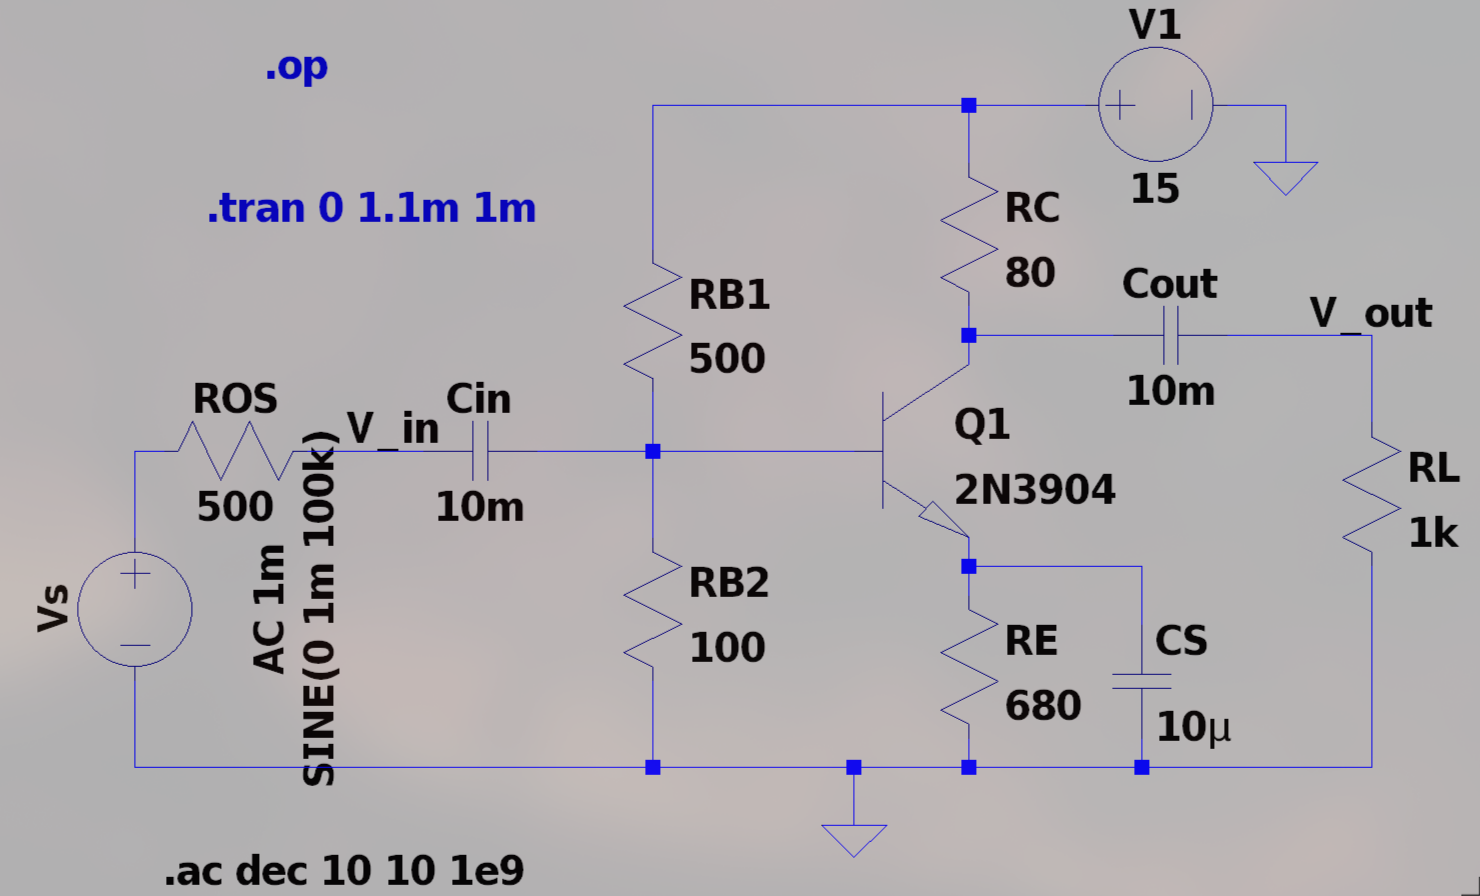
\includegraphics[width=0.7\linewidth]{figs/bjt_ce_ckt.png}
    \end{figure}
\subsubsection{DC Operating Point}
\begin{figure}[h!]
        \centering
        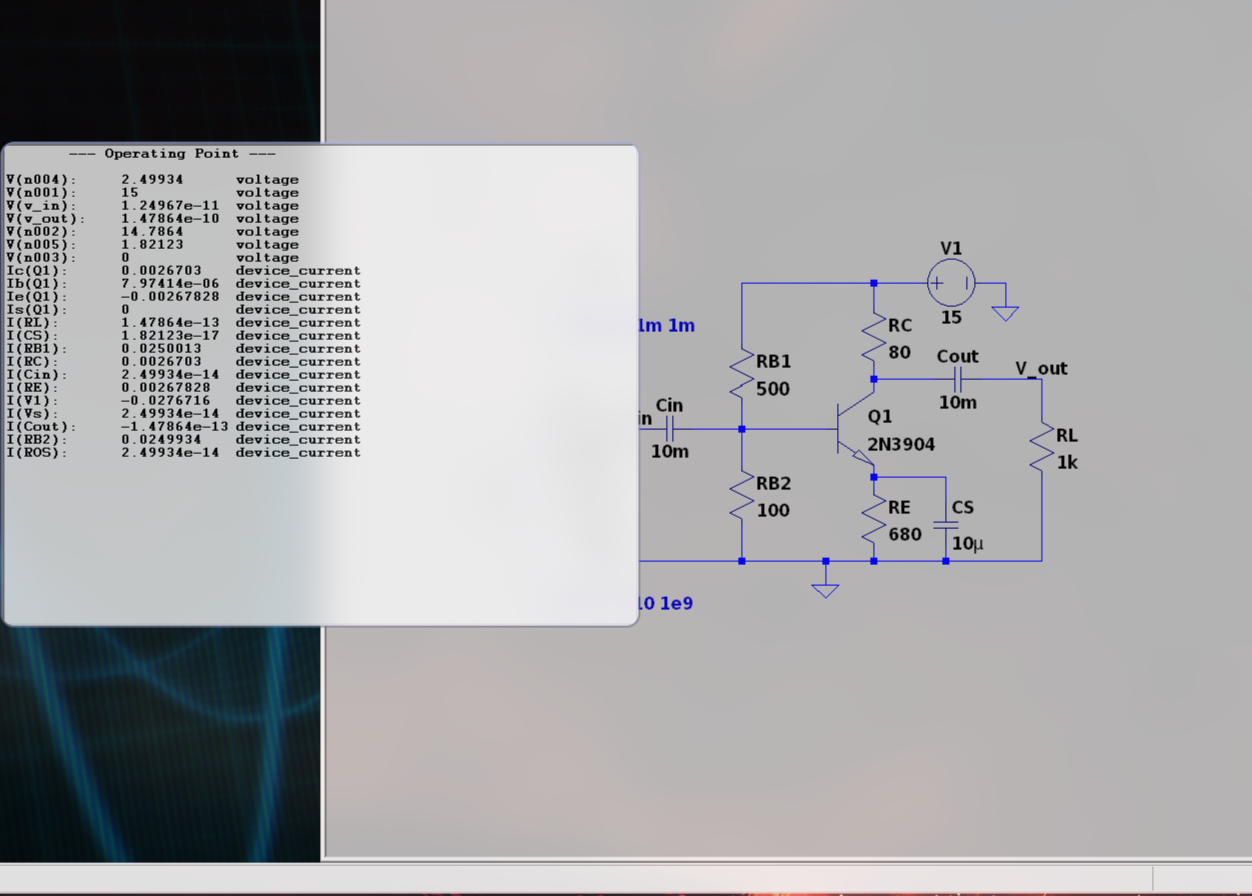
\includegraphics[width=0.7\linewidth]{figs/bjt_ce_op.png}
    \end{figure}
\pagebreak
\subsubsection{Midband Gain}
\begin{figure}[h!]
        \centering
        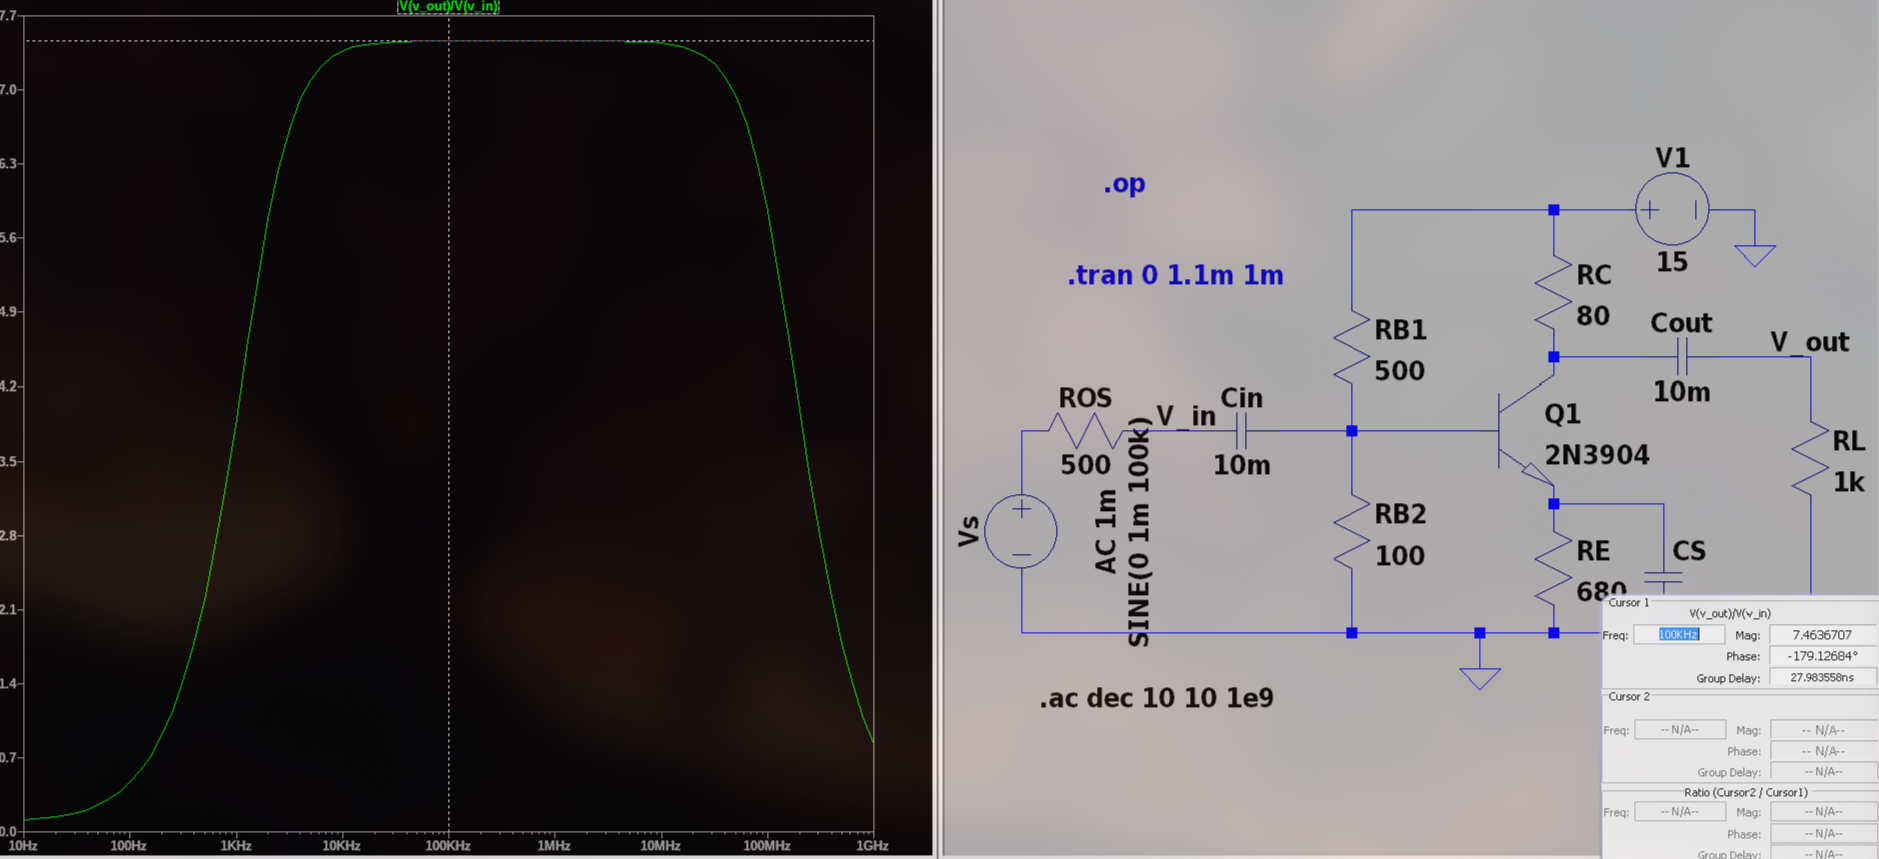
\includegraphics[width=0.7\linewidth]{figs/bjt_ce_mb.png}
    \end{figure}
\subsubsection{Bandwidth}
\begin{figure}[h!]
        \centering
        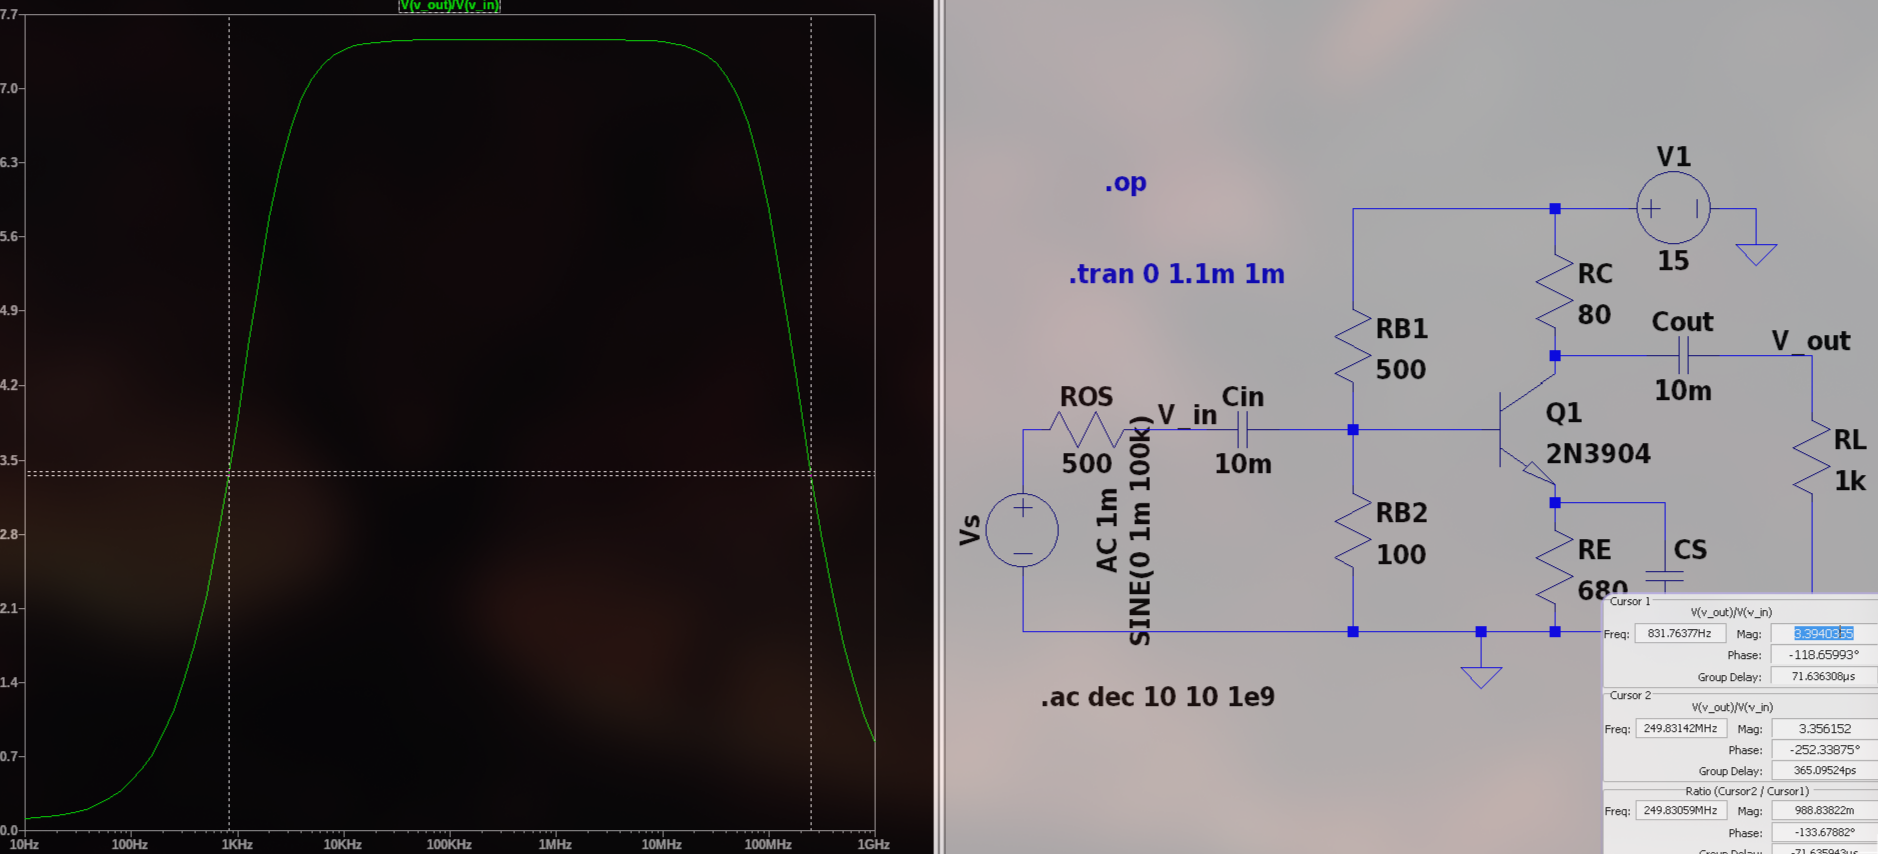
\includegraphics[width=0.7\linewidth]{figs/bjt_ce_bw.png}
    \end{figure}
\subsubsection{Transient}
\begin{figure}[h!]
        \centering
        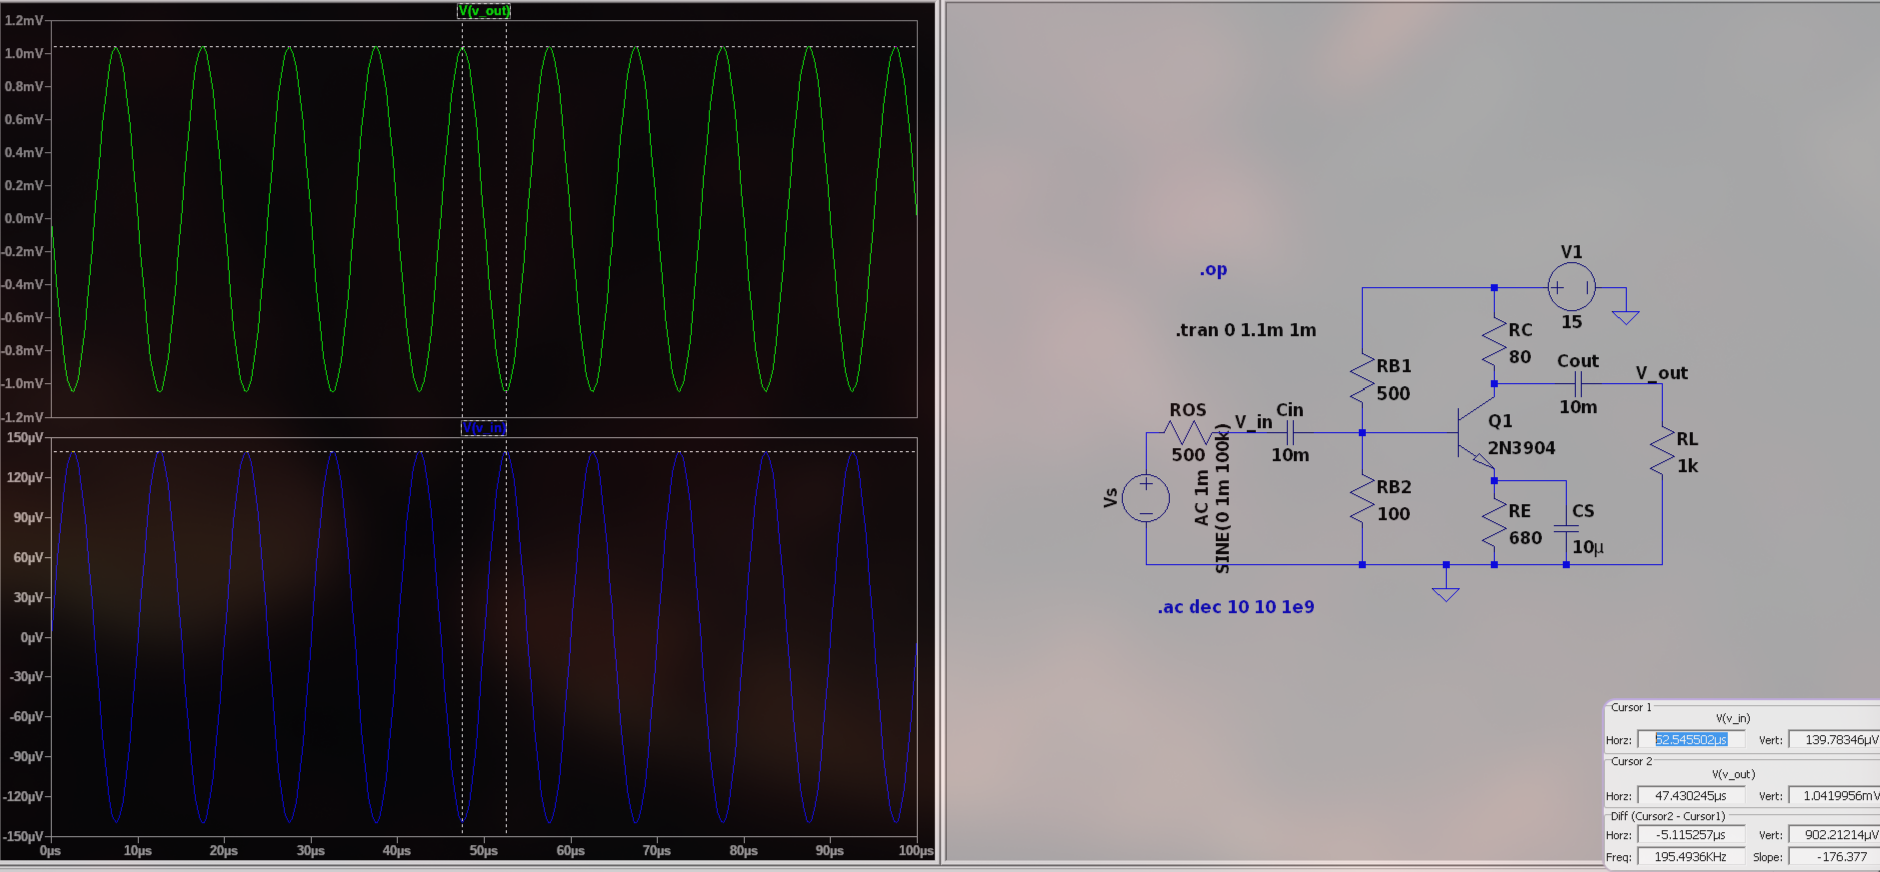
\includegraphics[width=0.7\linewidth]{figs/bjt_ce_tr.png}
    \end{figure}
        \pagebreak
\subsubsection{Input Resistance}
\begin{figure}[h!]
        \centering
        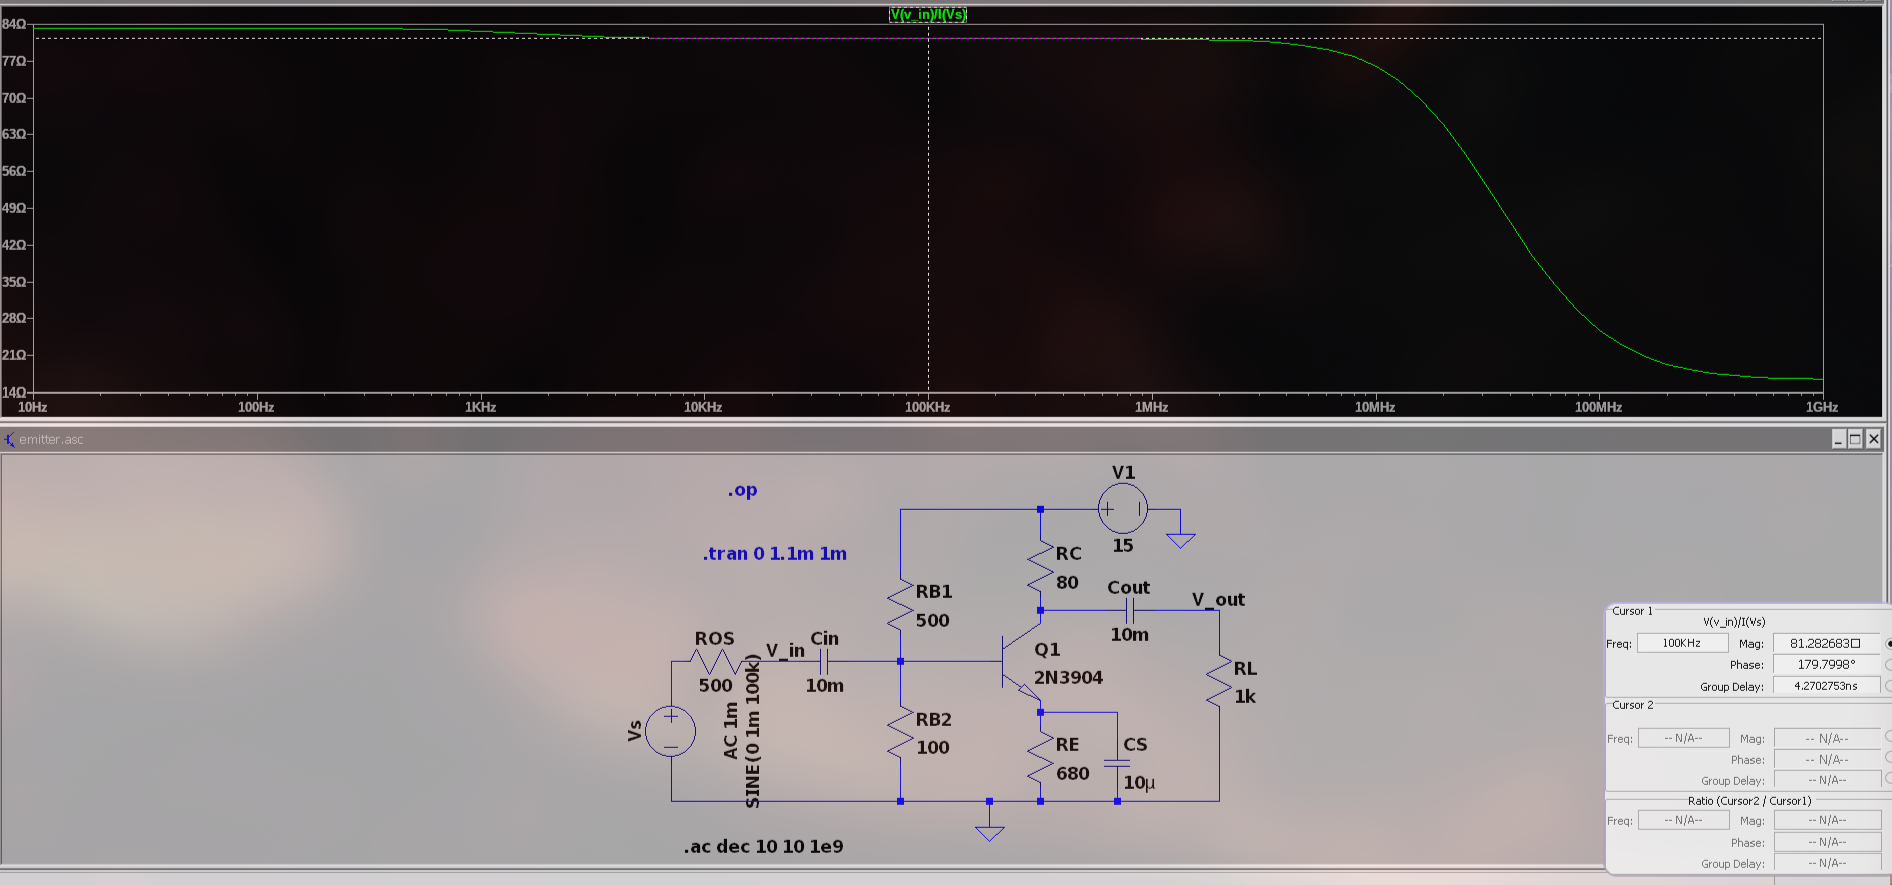
\includegraphics[width=0.7\linewidth]{figs/bjt_ce_rin.png}
    \end{figure}
\subsubsection{Output Resistance}
\begin{figure}[h!]
        \centering
        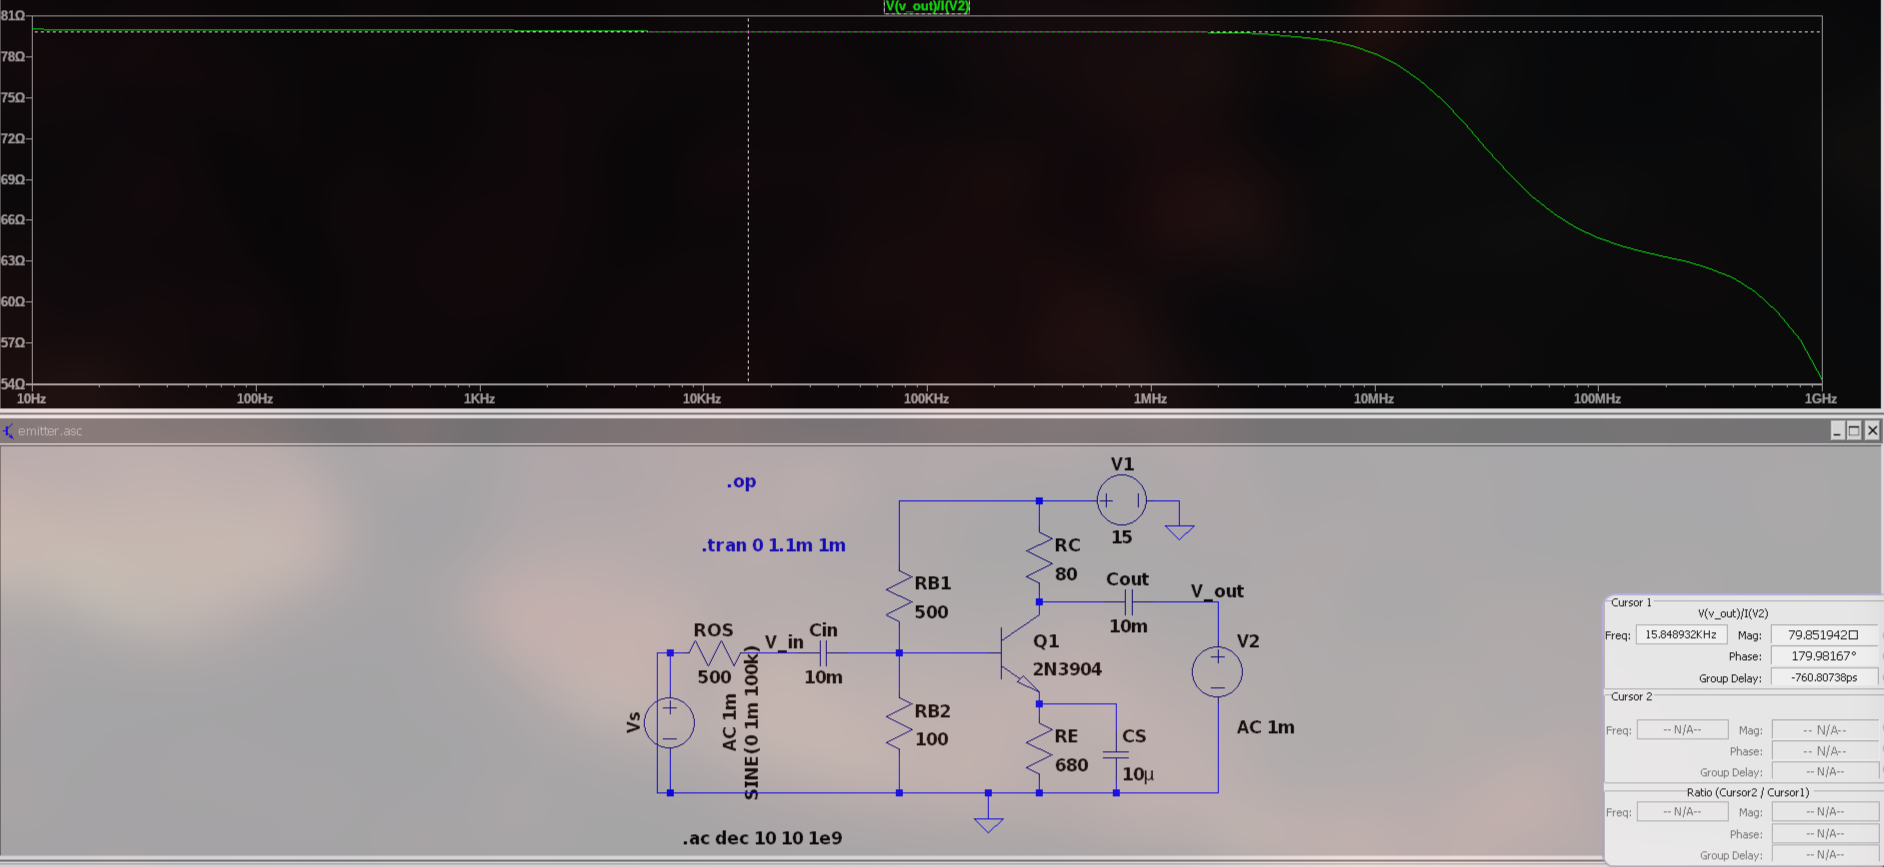
\includegraphics[width=0.7\linewidth]{figs/bjt_ce_rout.png}
    \end{figure}

\subsubsection{Theory}
\begin{enumerate}
    \item Transconductance $g_m = \frac{I_C}{V_T}$  (where $V_T = \frac{kT}{q}$)
    \item Input Resistance $R_i = R_{B1} \parallel R_{B2} \parallel r_{\pi} $
    \item $r_{\pi} = \frac{\beta}{g_m}$ 
    \item $\beta = \frac{I_C}{I_B}$
    \item Output Resistance $R_o = R_C $ 
    \item Voltage gain $A = \frac{V_{in}}{V_{out}} = g_m \brak{R_C \parallel R_L}$ 
\end{enumerate} 
\subsubsection{Data}
\begin{tabular}{|c|c|c|c|c|c|c|}
\hline
\makecell{\textbf{Midband gain} \\ \textbf{(graph)}} & \makecell{\textbf{Midband gain} \\ \textbf{(theory)}} & \makecell{$\mathbf{R_i}$ \\ \textbf{(graph)}} & \makecell{{$\mathbf{R_i}$} \\ \textbf{(theory)}} & \makecell{{$\mathbf{R_o}$} \\ \textbf{(graph)}} & \makecell{{$\mathbf{R_o}$} \\ \textbf{(theory)}} & \textbf{Bandwidth} \\
\hline
$7.4636707$ & $7.6435$ & $81.282683\Omega$ & $81.24784\Omega$& $79.85194\Omega$ & $74.074074\Omega$ & $249.8305MHz$ \\
\hline
\end{tabular}
\pagebreak
\subsection{Common Collector}
\subsubsection{Circuit}
\begin{figure}[h!]
        \centering
        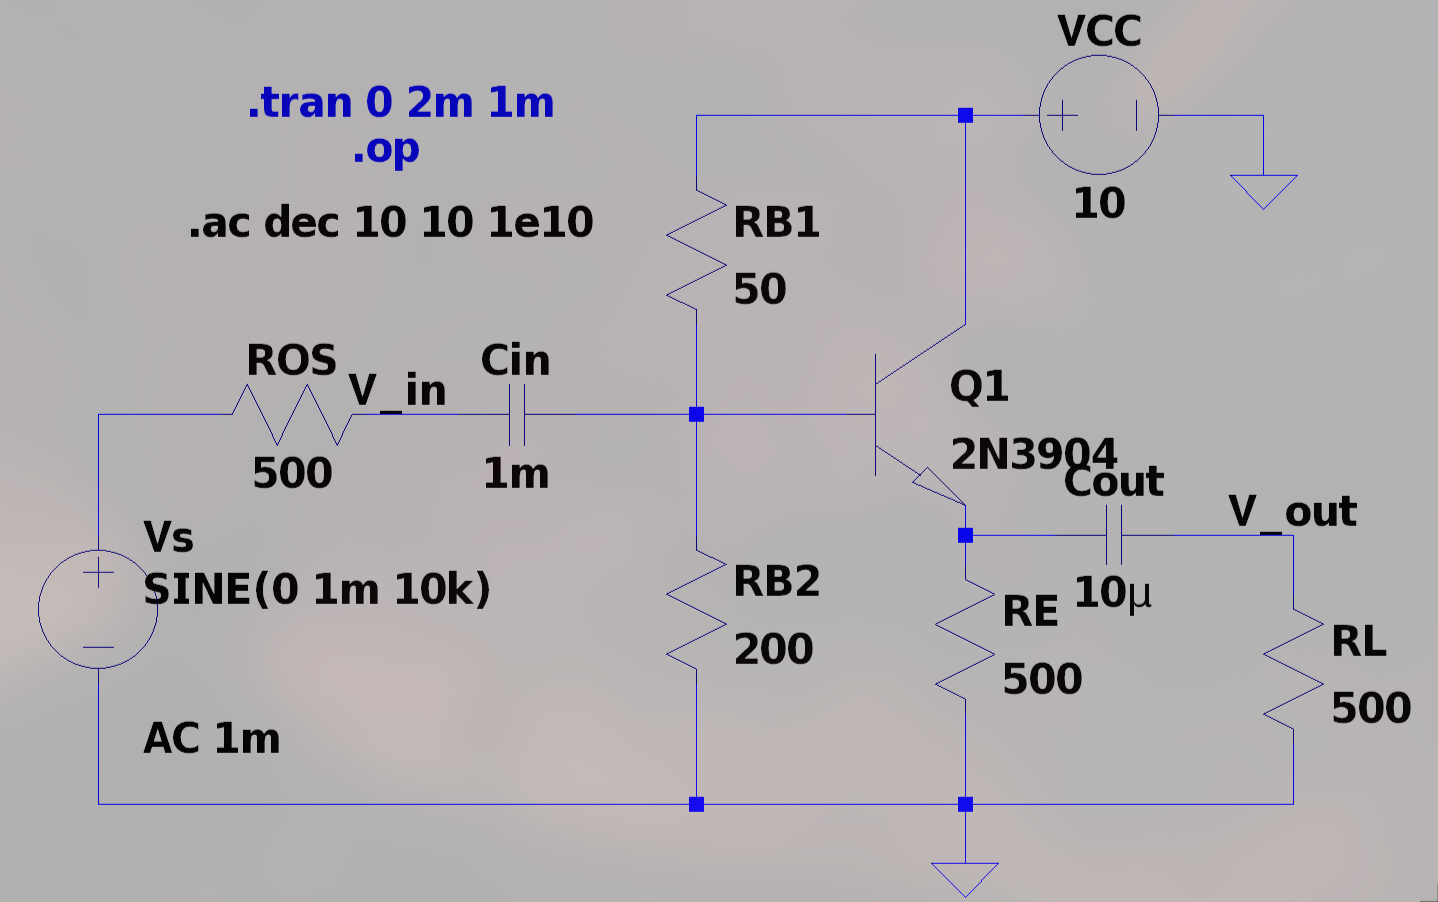
\includegraphics[width=0.7\linewidth]{figs/bjt_cc_ckt.png}
    \end{figure}
\subsubsection{DC Operating Point}
\begin{figure}[h!]
        \centering
        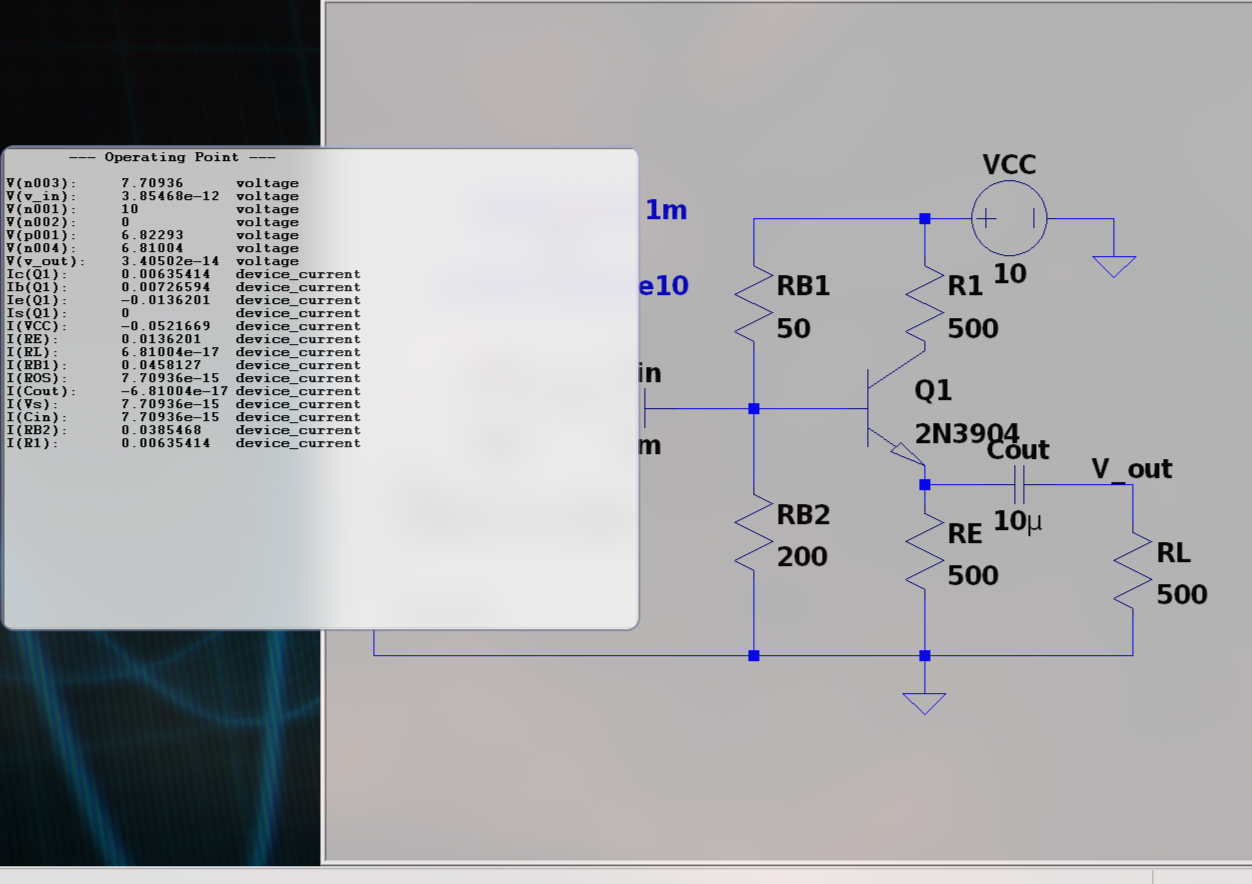
\includegraphics[width=0.7\linewidth]{figs/bjt_cc_op.png}
    \end{figure}
\pagebreak
\subsubsection{Midband Gain}
\begin{figure}[h!]
        \centering
        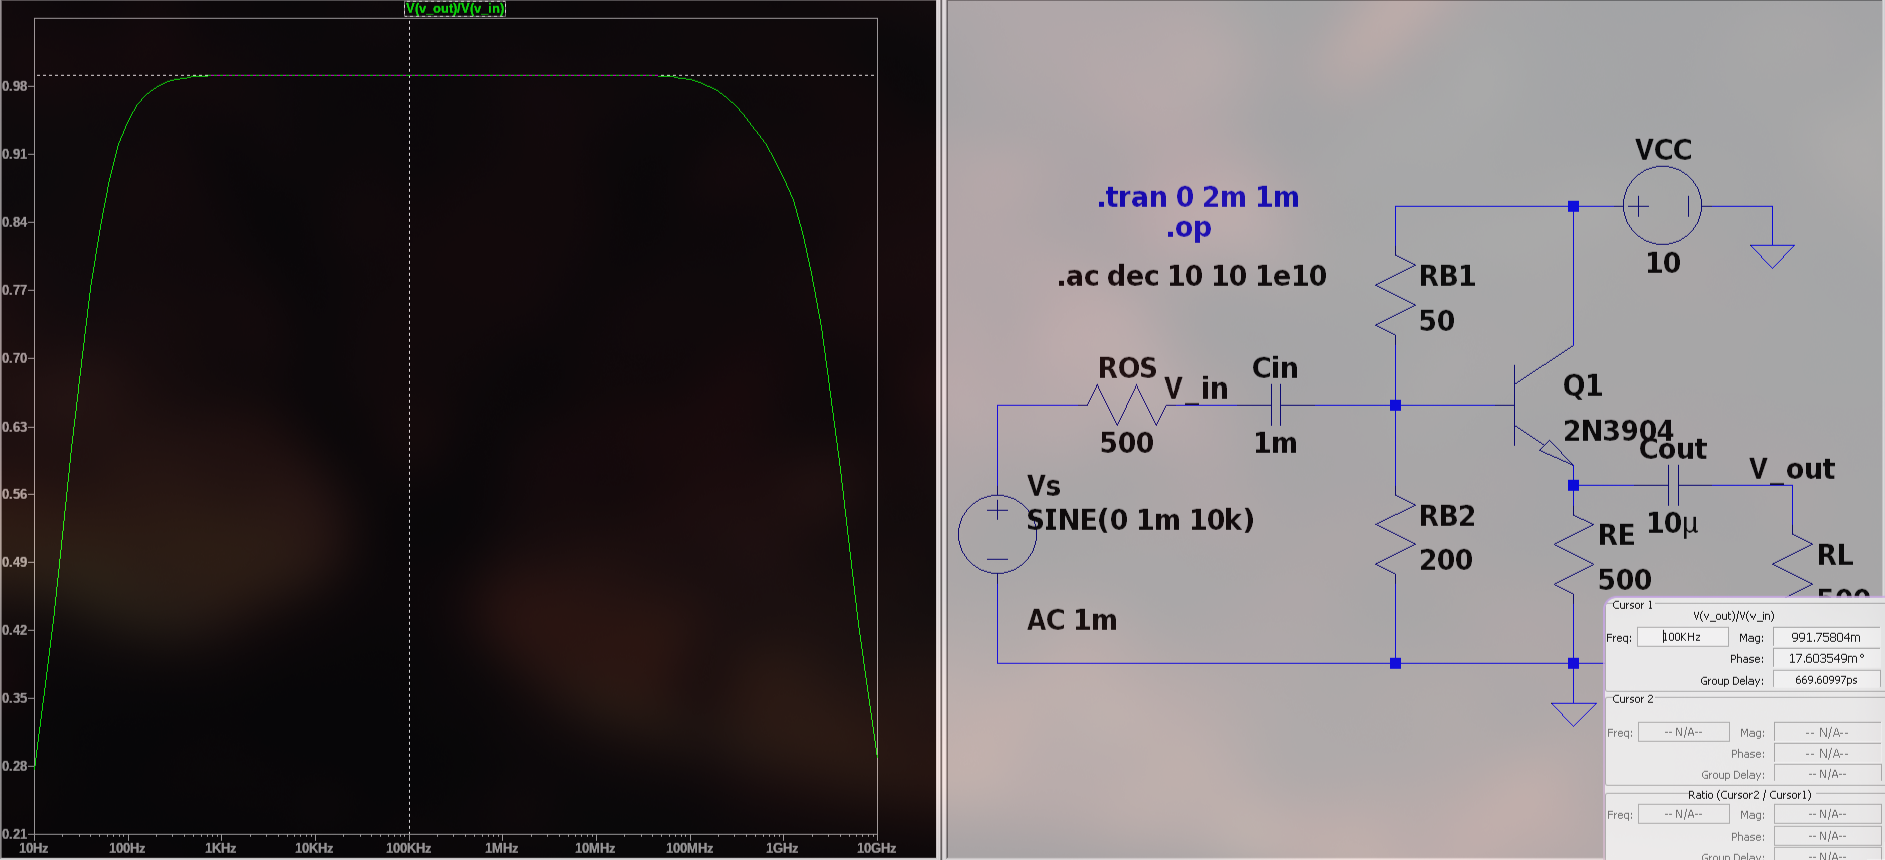
\includegraphics[width=0.7\linewidth]{figs/bjt_cc_mb.png}
    \end{figure}
\subsubsection{Bandwidth}
\begin{figure}[h!]
        \centering
        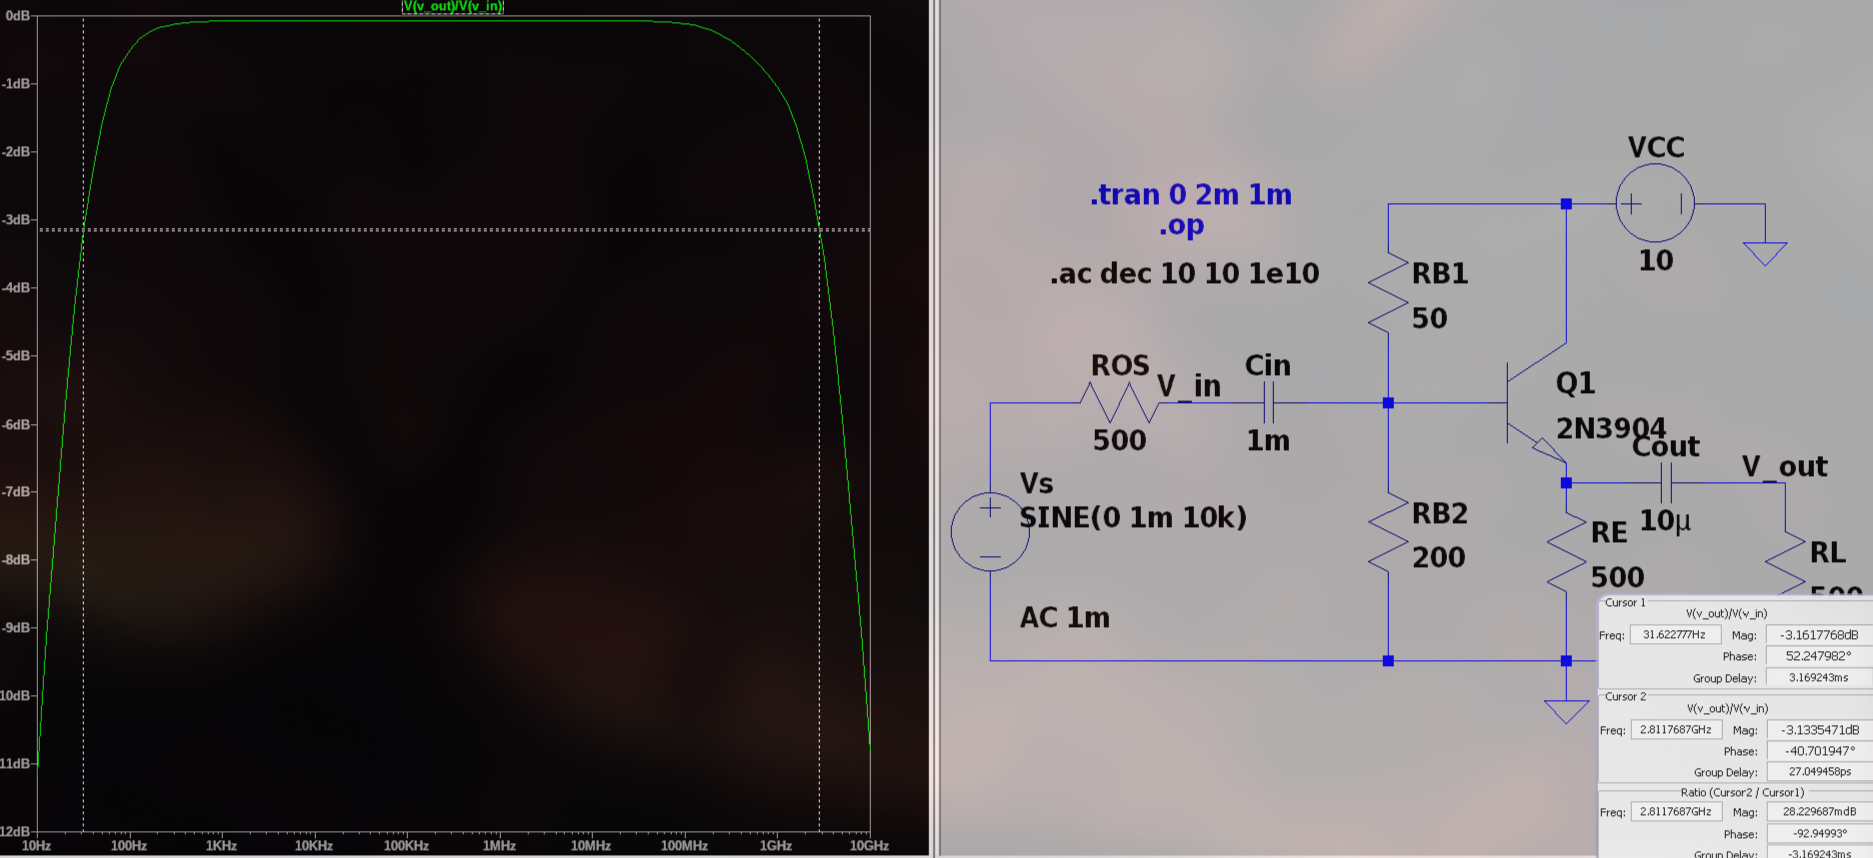
\includegraphics[width=0.7\linewidth]{figs/bjt_cc_bw.png}
    \end{figure}
\subsubsection{Transient}
\begin{figure}[h!]
        \centering
        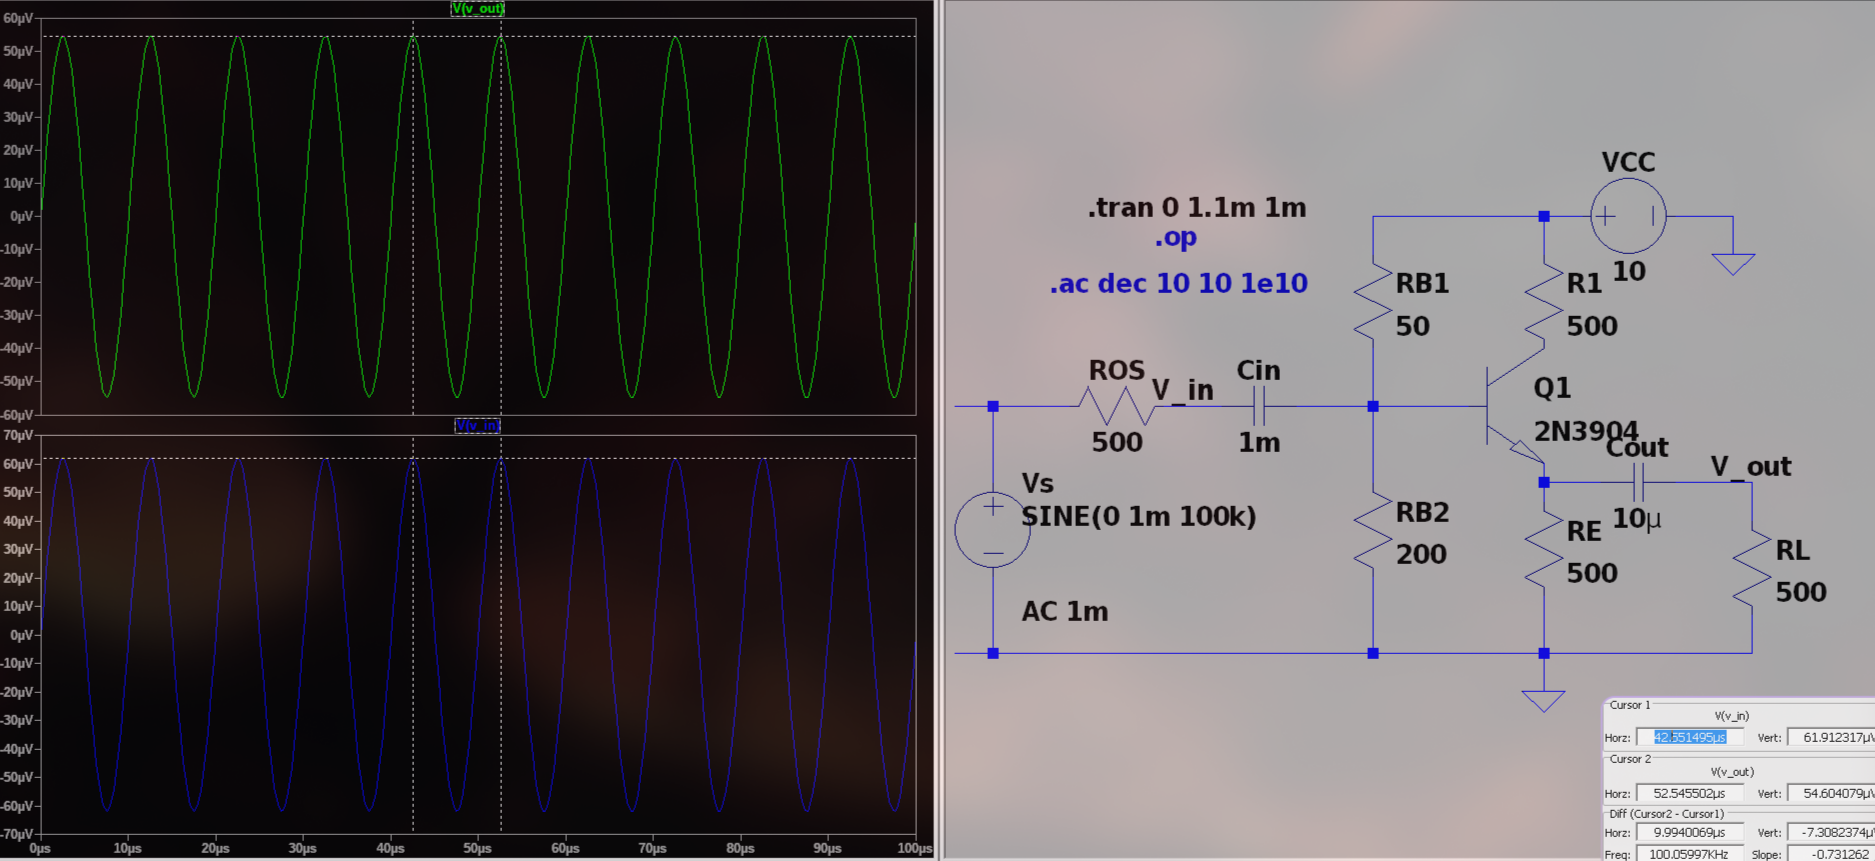
\includegraphics[width=0.7\linewidth]{figs/bjt_cc_tr.png}
    \end{figure}
            \pagebreak
\subsubsection{Input Resistance}
\begin{figure}[h!]
        \centering
        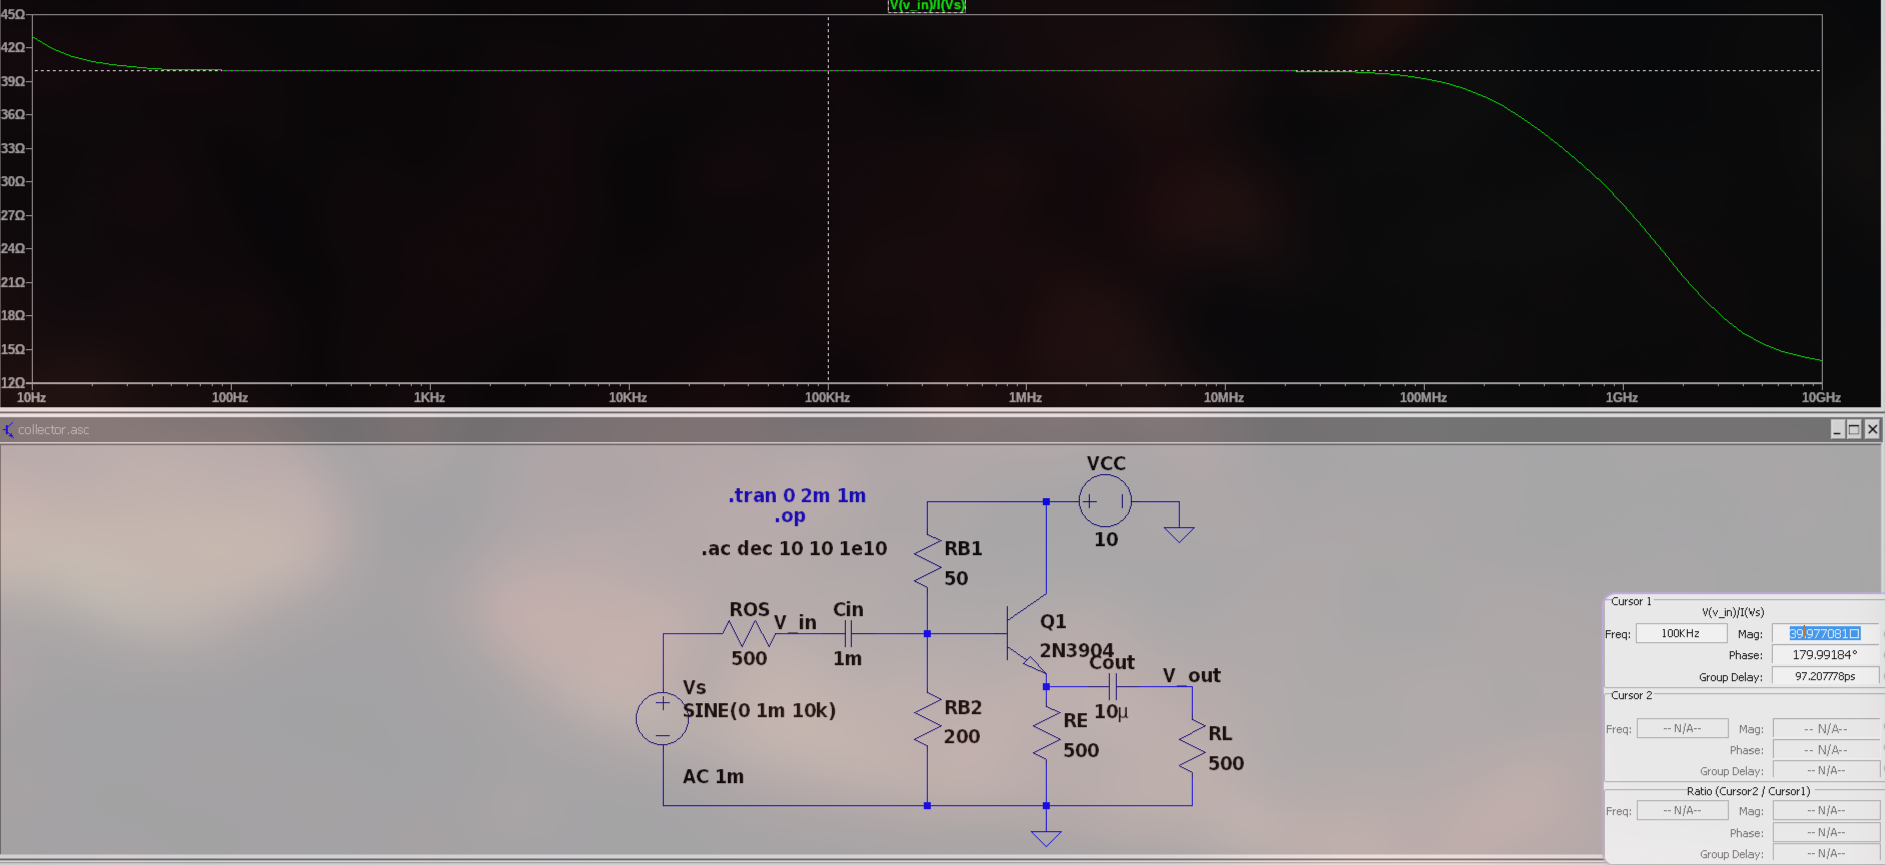
\includegraphics[width=0.7\linewidth]{figs/bjt_cc_rin.png}
    \end{figure}
\subsubsection{Output Resistance}
\begin{figure}[h!]
        \centering
        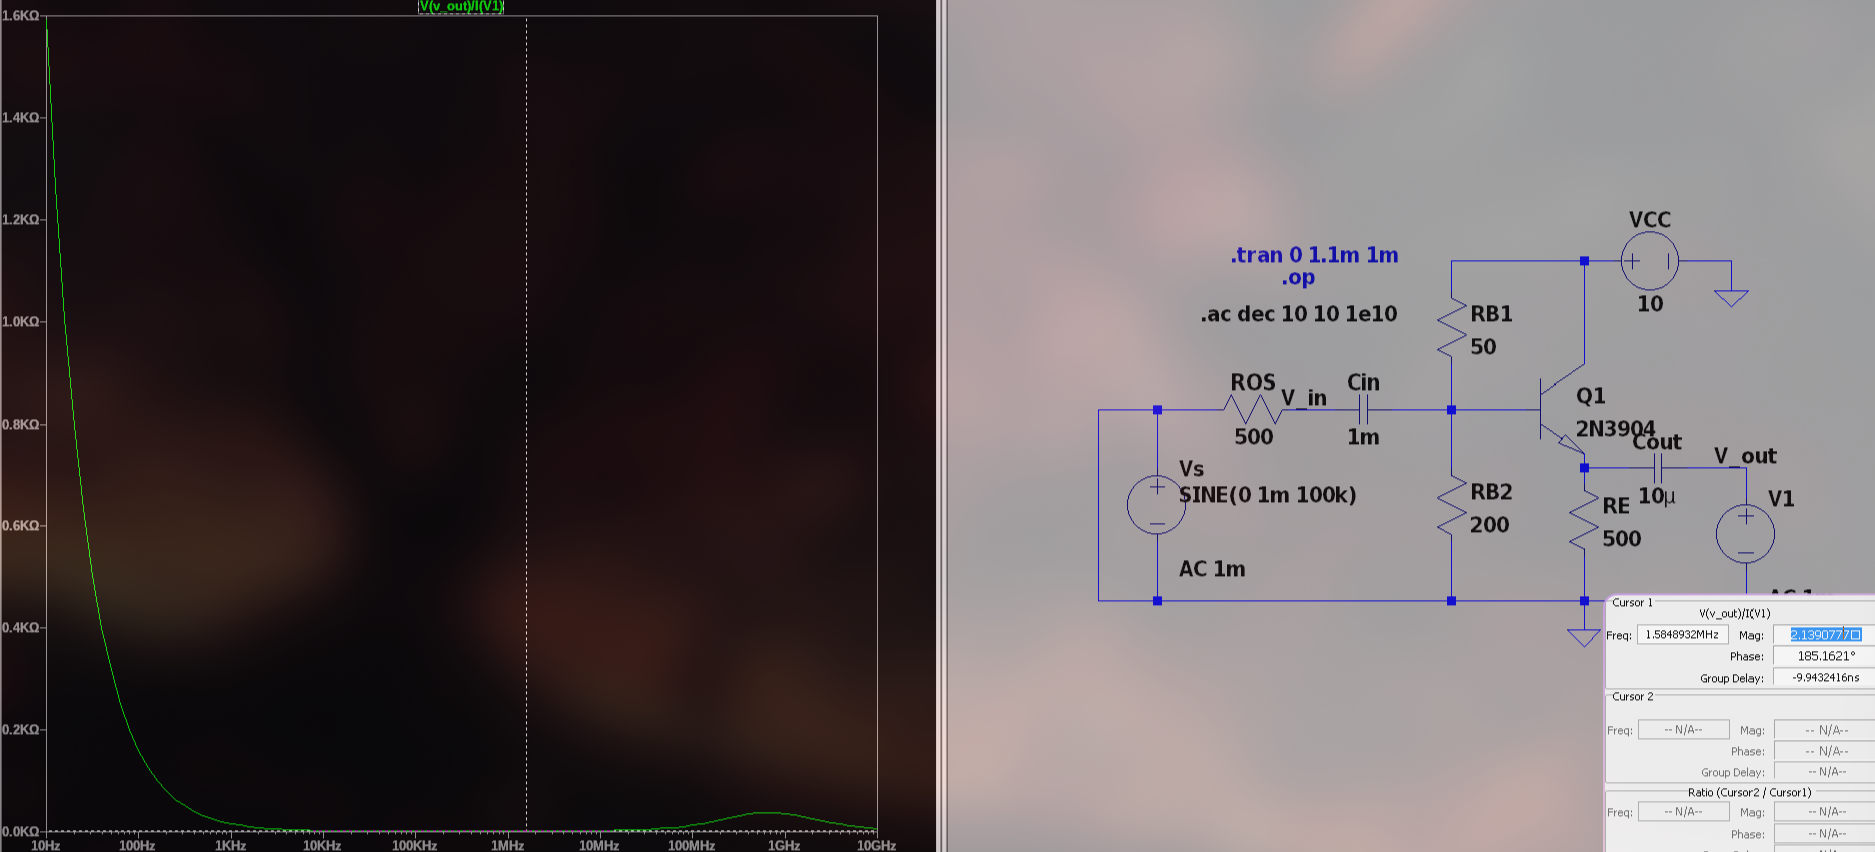
\includegraphics[width=0.7\linewidth]{figs/bjt_cc_rout.png}
    \end{figure}

\subsubsection{Theory}
\begin{enumerate}
    \item $r_e^{\prime} = \frac{V_T}{I_E}$  (where $V_T = \frac{kT}{q}$)
    \item Input Resistance $R_i = R_{B1} \parallel R_{B2} || \beta(R_E \parallel R_L) $
    \item Output Resistance $R_o = r_e^{\prime} \parallel R_E \parallel R_L$ 
    \item Voltage gain $A = \frac{V_{in}}{V_{out}} = \frac{R_E}{R_E + r_e^{\prime}}$ 
\end{enumerate} 
\begin{tabular}{|c|c|c|c|c|c|c|}
\hline
\makecell{\textbf{Midband gain} \\ \textbf{(graph)}} & \makecell{\textbf{Midband gain} \\ \textbf{(theory)}} & \makecell{$\mathbf{R_i}$ \\ \textbf{(graph)}} & \makecell{{$\mathbf{R_i}$} \\ \textbf{(theory)}} & \makecell{{$\mathbf{R_o}$} \\ \textbf{(graph)}} & \makecell{{$\mathbf{R_o}$} \\ \textbf{(theory)}} & \textbf{Bandwidth} \\
\hline
$0.991758$ & $0.99293$ & $39.977081\Omega$ & $39.978354\Omega $& $2.139077\Omega$ & $1.766766\Omega$ & $2.8117GHz$ \\
\hline
\end{tabular}
\pagebreak
\subsection{Common Base}
\subsubsection{Circuit}
\begin{figure}[h!]
        \centering
        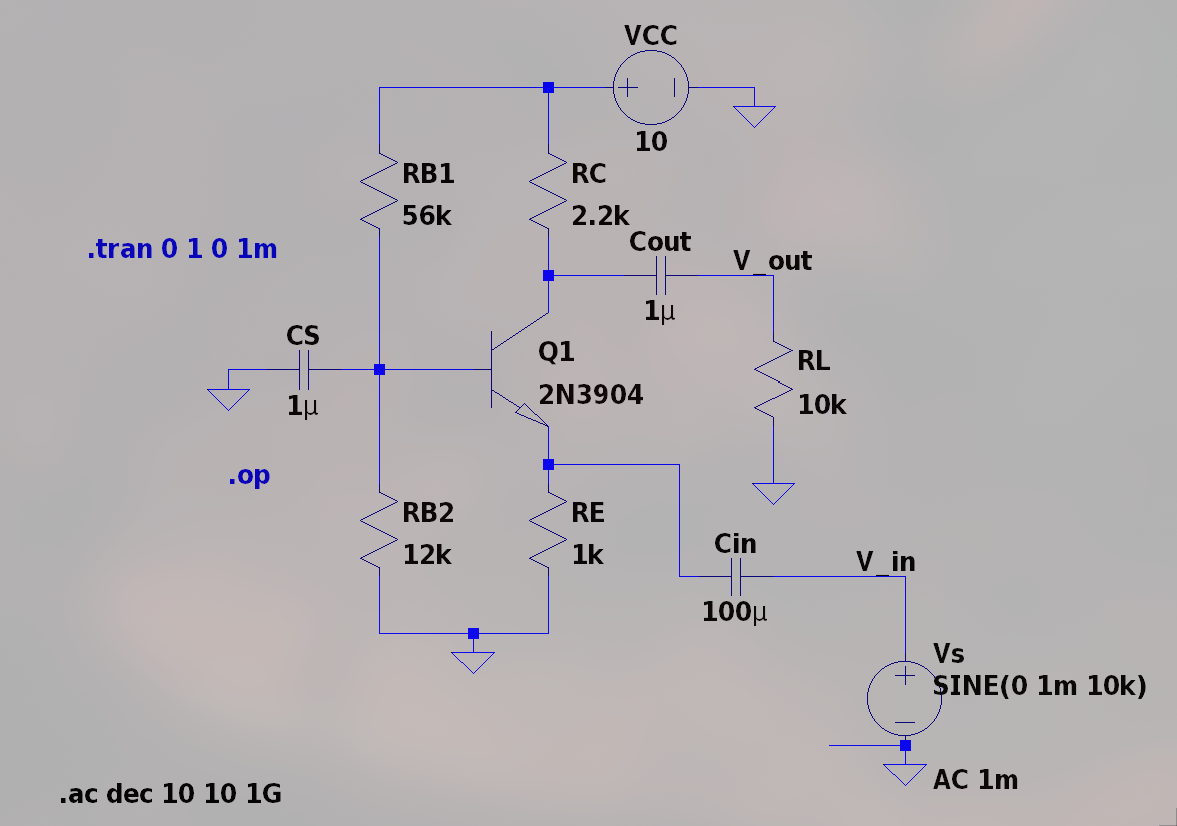
\includegraphics[width=0.7\linewidth]{figs/bjt_cb_ckt.png}
    \end{figure}
\subsubsection{DC Operating Point}
\begin{figure}[h!]
        \centering
        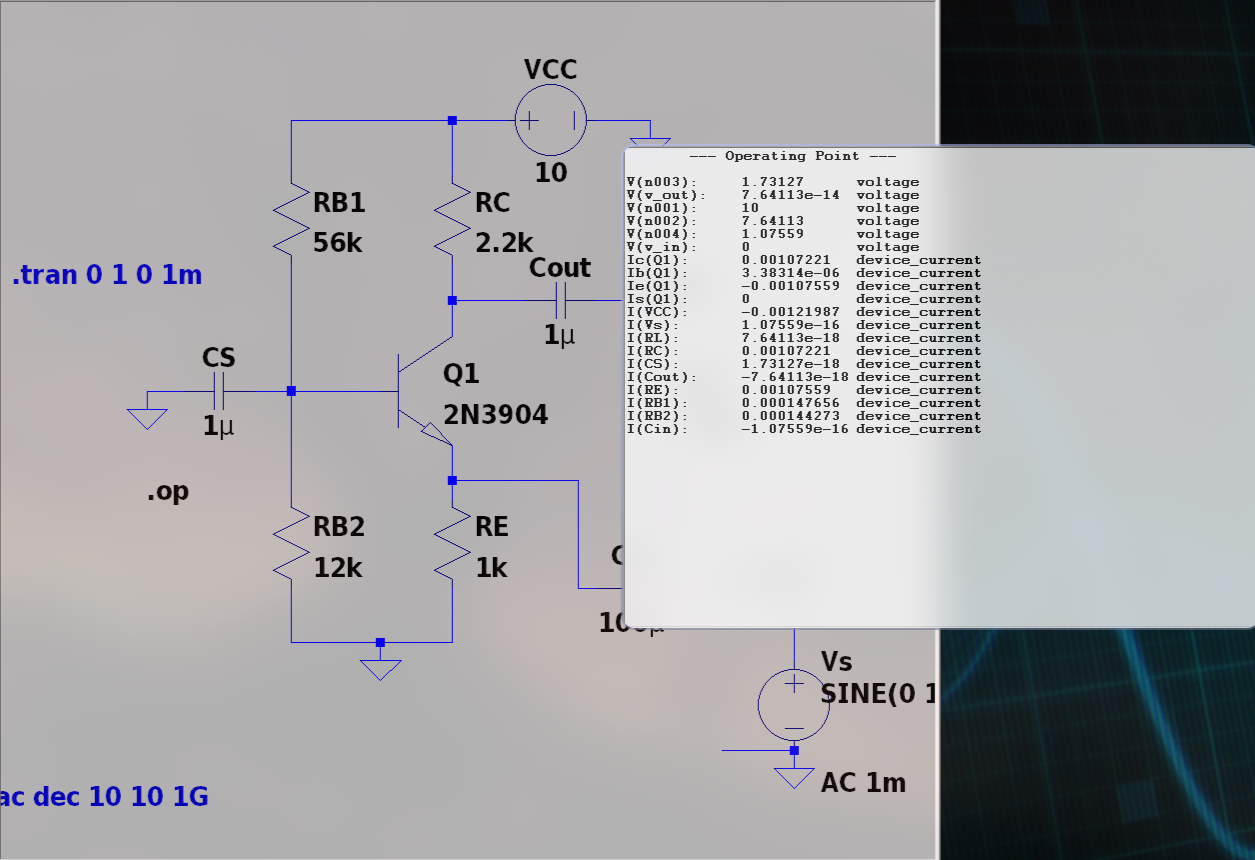
\includegraphics[width=0.7\linewidth]{figs/bjt_cb_op.png}
    \end{figure}
\pagebreak
\subsubsection{Midband Gain}
\begin{figure}[h!]
        \centering
        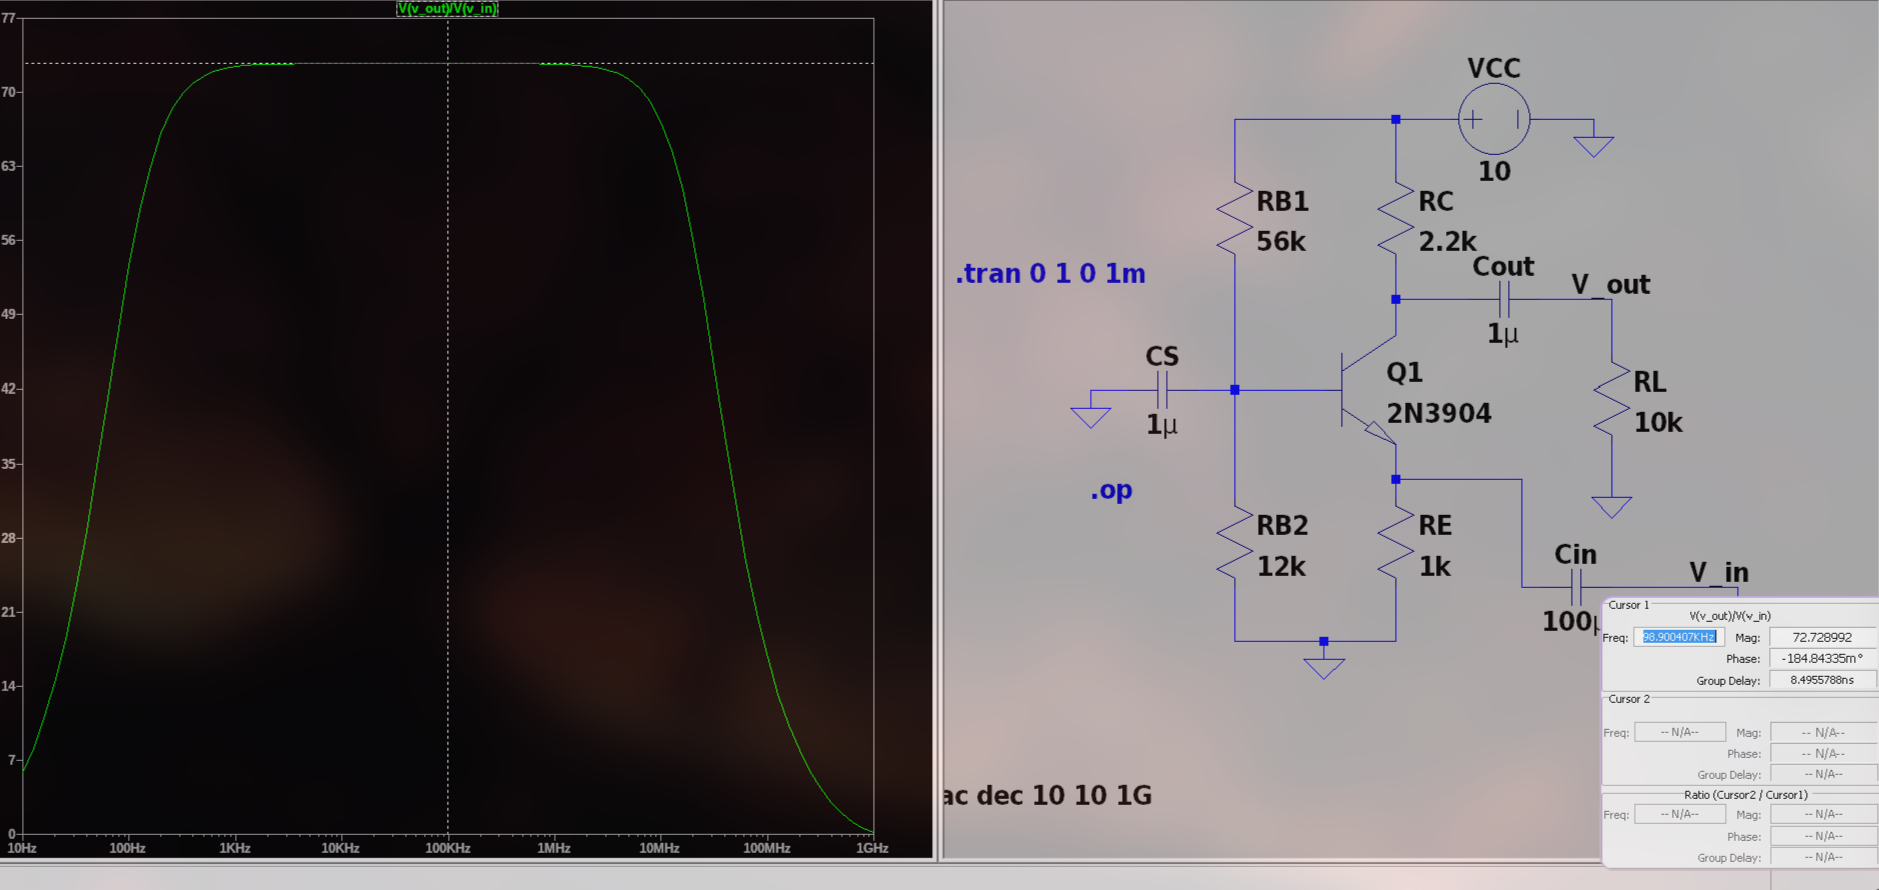
\includegraphics[width=0.7\linewidth]{figs/bjt_cb_mb.png}
    \end{figure}
\subsubsection{Bandwidth}
\begin{figure}[h!]
        \centering
        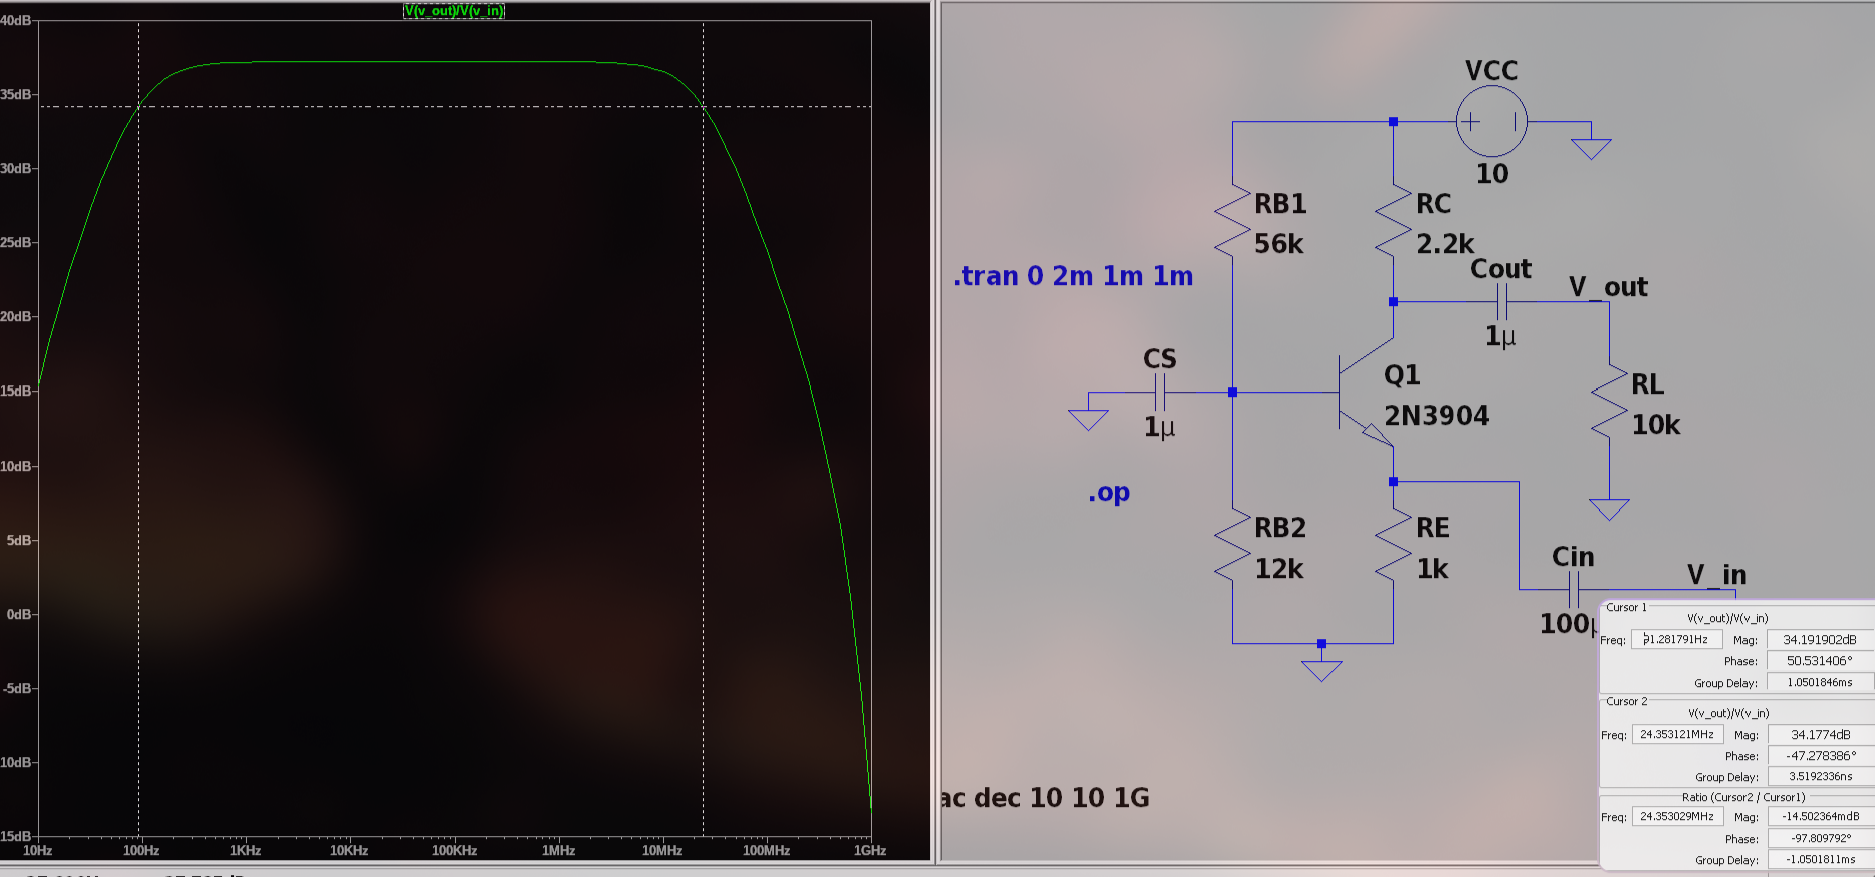
\includegraphics[width=0.7\linewidth]{figs/bjt_cb_bw.png}
    \end{figure}
\subsubsection{Transient}
\begin{figure}[h!]
        \centering
        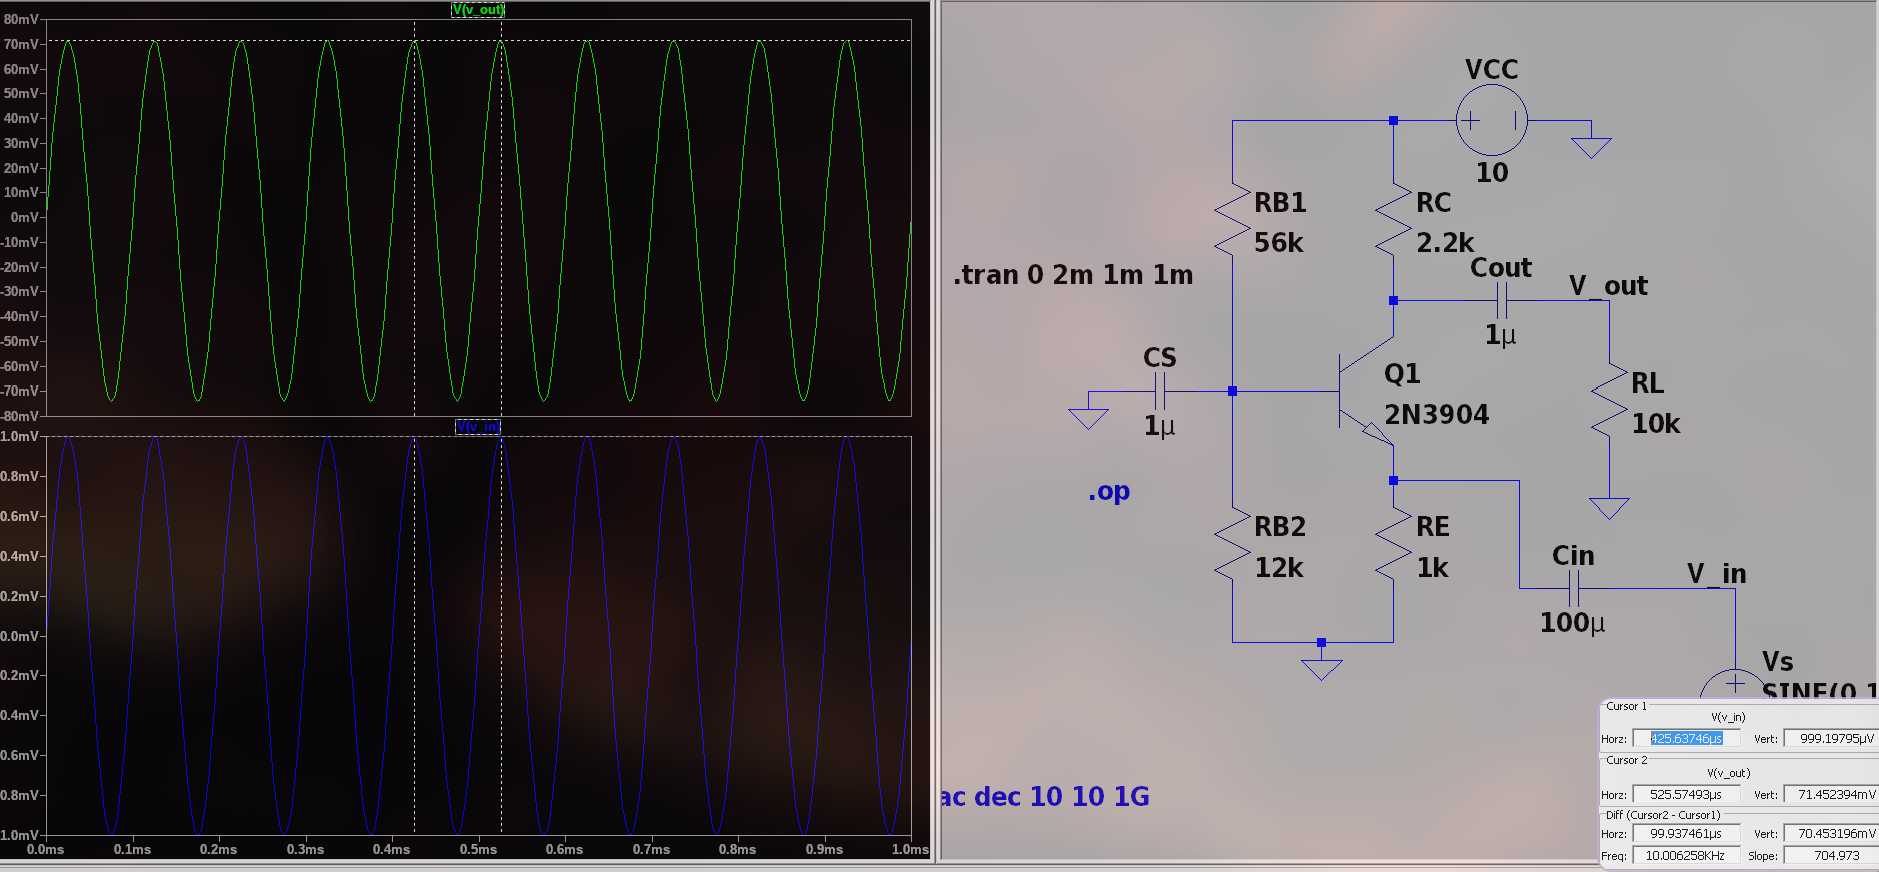
\includegraphics[width=0.7\linewidth]{figs/bjt_cb_tr.png}
    \end{figure}
            \pagebreak
\subsubsection{Input Resistance}
\begin{figure}[h!]
        \centering
        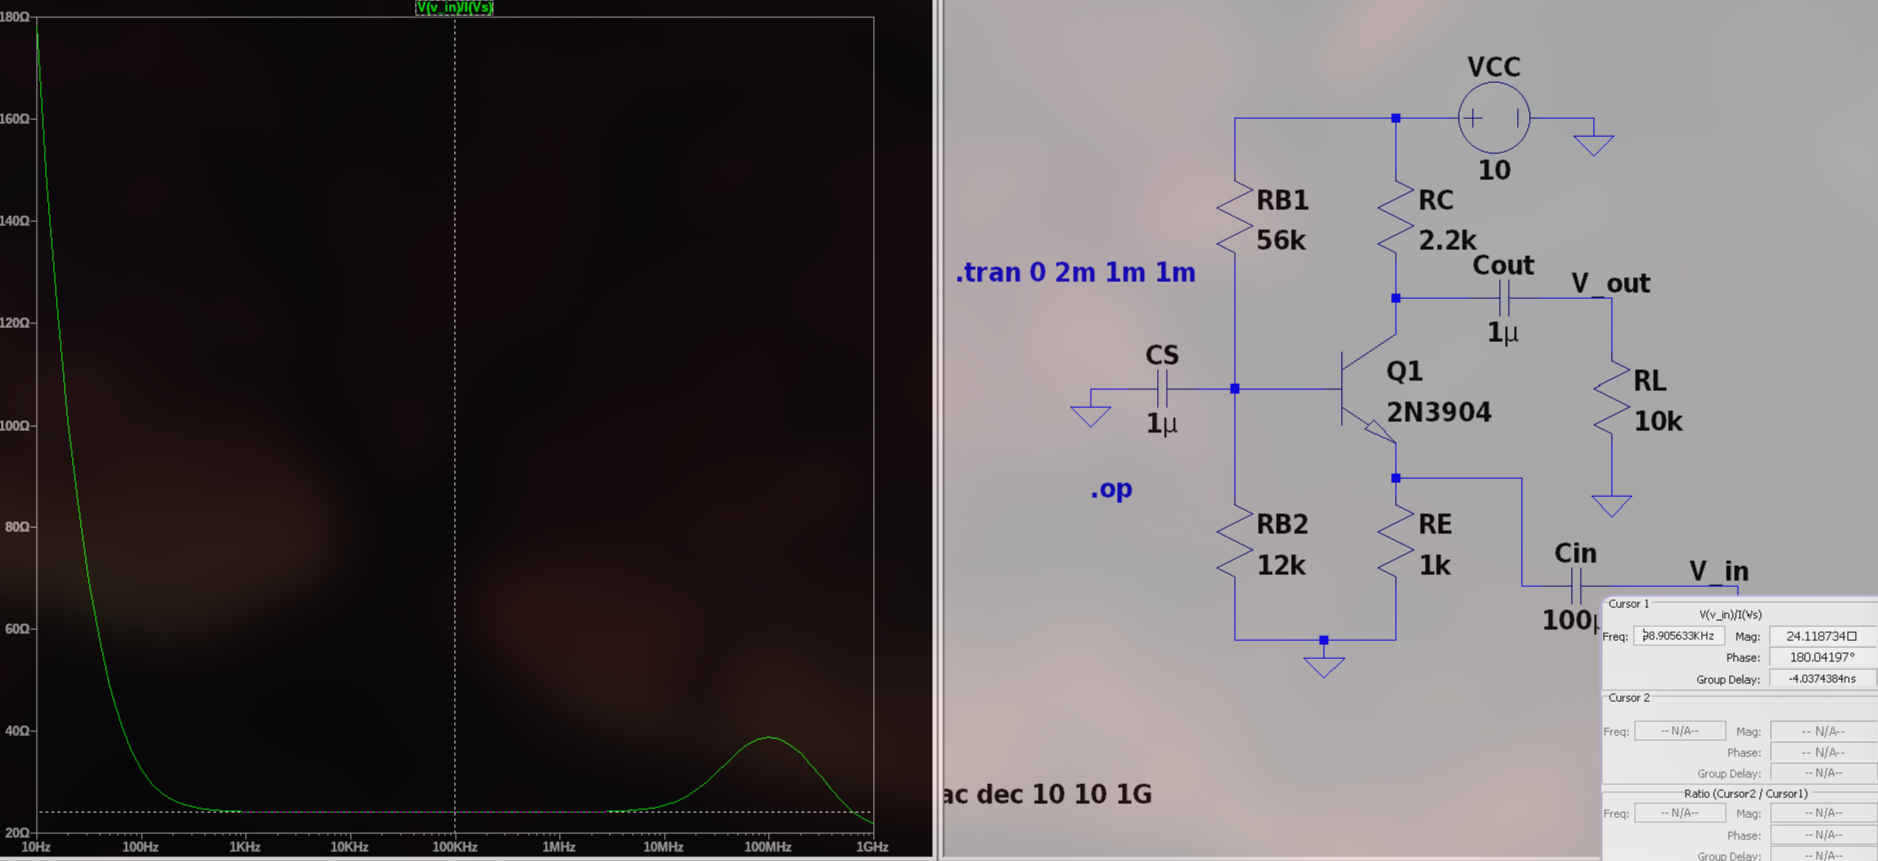
\includegraphics[width=0.7\linewidth]{figs/bjt_cb_rin.png}
    \end{figure}
\subsubsection{Output Resistance}
\begin{figure}[h!]
        \centering
        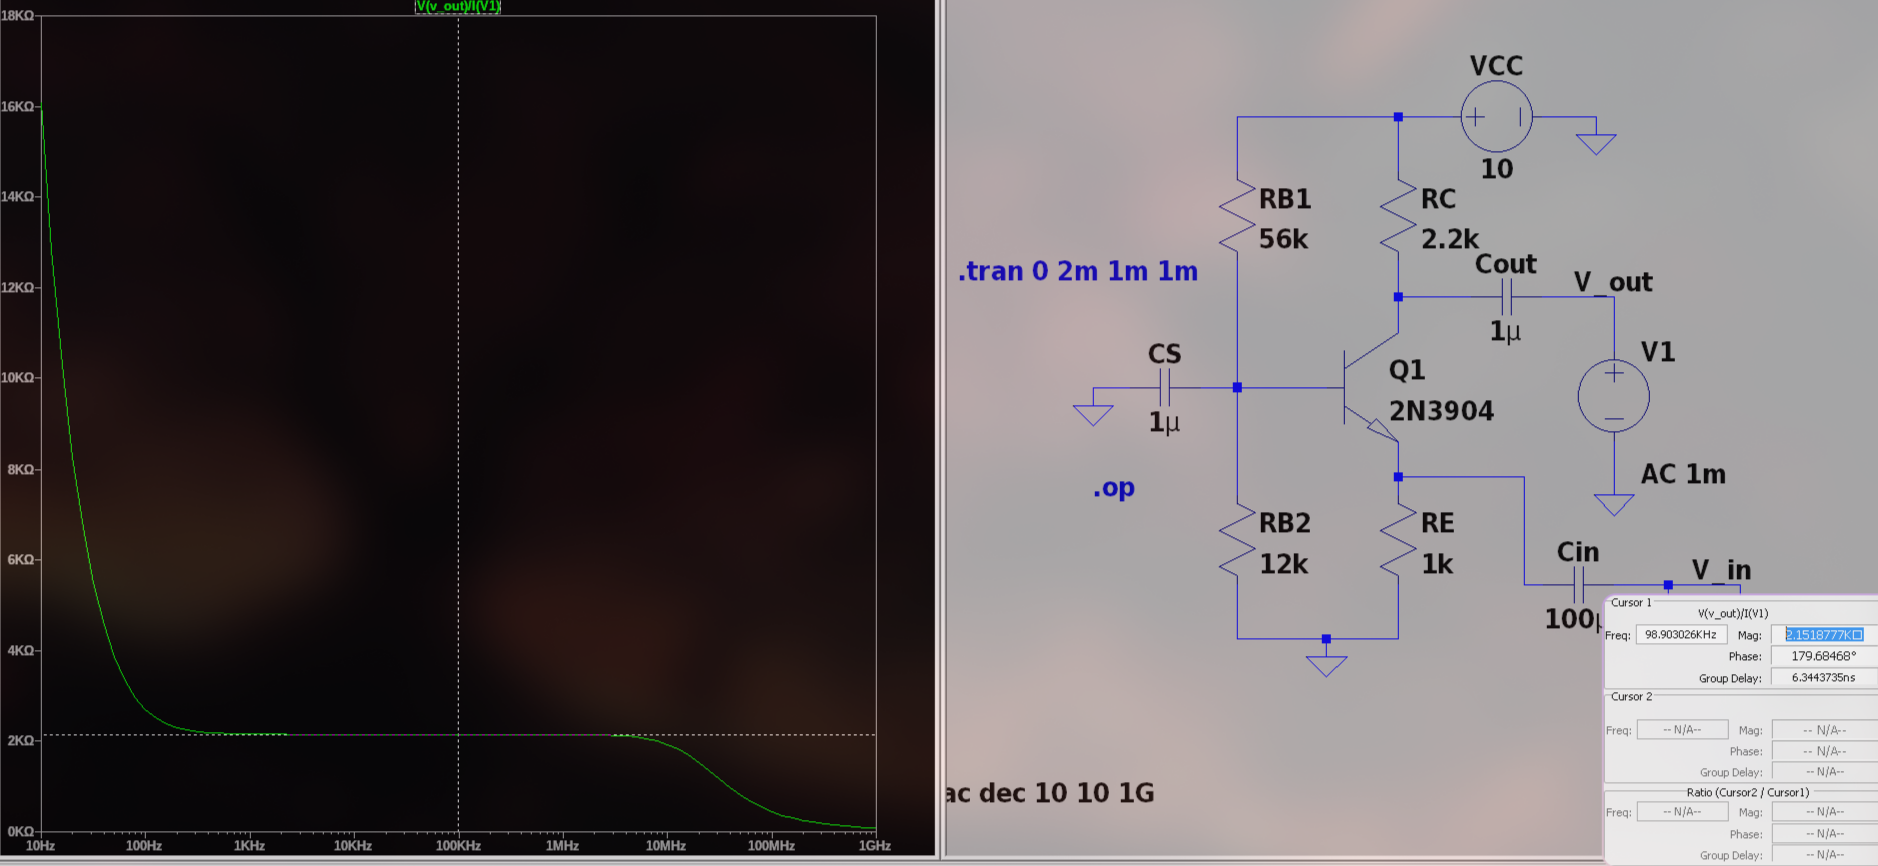
\includegraphics[width=0.7\linewidth]{figs/bjt_cb_rout.png}
    \end{figure}

\subsubsection{Theory}
\begin{enumerate}
    \item $r_e^{\prime} = \frac{V_T}{I_E}$  (where $V_T = \frac{kT}{q}$) 
    \item Input Resistance $R_i = r_e^{\prime} \parallel R_{E} $
    \item Output Resistance $R_o = R_C $ 
    \item Voltage gain $A = \frac{V_{in}}{V_{out}} = \frac{R_C \parallel R_L}{r_e^{\prime}}$ 
\end{enumerate} 
\subsubsection{Data}
\begin{tabular}{|c|c|c|c|c|c|c|}
\hline
\makecell{\textbf{Midband gain} \\ \textbf{(graph)}} & \makecell{\textbf{Midband gain} \\ \textbf{(theory)}} & \makecell{$\mathbf{R_i}$ \\ \textbf{(graph)}} & \makecell{{$\mathbf{R_i}$} \\ \textbf{(theory)}} & \makecell{{$\mathbf{R_o}$} \\ \textbf{(graph)}} & \makecell{{$\mathbf{R_o}$} \\ \textbf{(theory)}} & \textbf{Bandwidth} \\
\hline
$72.728992$ & $74.95367$ & $24.11873\Omega$ & $24.0585774\Omega$& $2.1518777k\Omega$ & $2.2 k\Omega$ & $24.353MHz$ \\
\hline
\end{tabular}
\end{document}